\section{Amplificador ideal realimentado por tensión (VFA)}
\subsection*{Introducción}
El modelo asumido en la Figura~\ref{fig:1.1} describe con bastante exactitud el comportamiento con pequeña señal de un A.O.\ clásico. Es importante destacar el orden de magnitud de los parámetros involucrados en el modelo asumido. Así, la impedancia de entrada de modo diferencial ($Z_{id}$) es muy elevada, siendo su componente resistiva superior al M$\Omega$ y la capacitiva apenas unos pocos picofaradios; de igual manera la impedancia de modo común ($Z_c$), cuyos valores son mayores a aquella en uno o dos órdenes de magnitud. En cambio, la impedancia de salida es muy baja (decenas de $\Omega$). El generador controlado de salida ($A(s)$) tiene dos componentes: la de modo diferencial $A_d(s)$, muy elevada (típico 100 dB), y la de modo común muy baja, definida generalmente a través de la relación de rechazo de modo común ($RRMC=A_d/A_c$).
\begin{figure}[H]
    \centering
    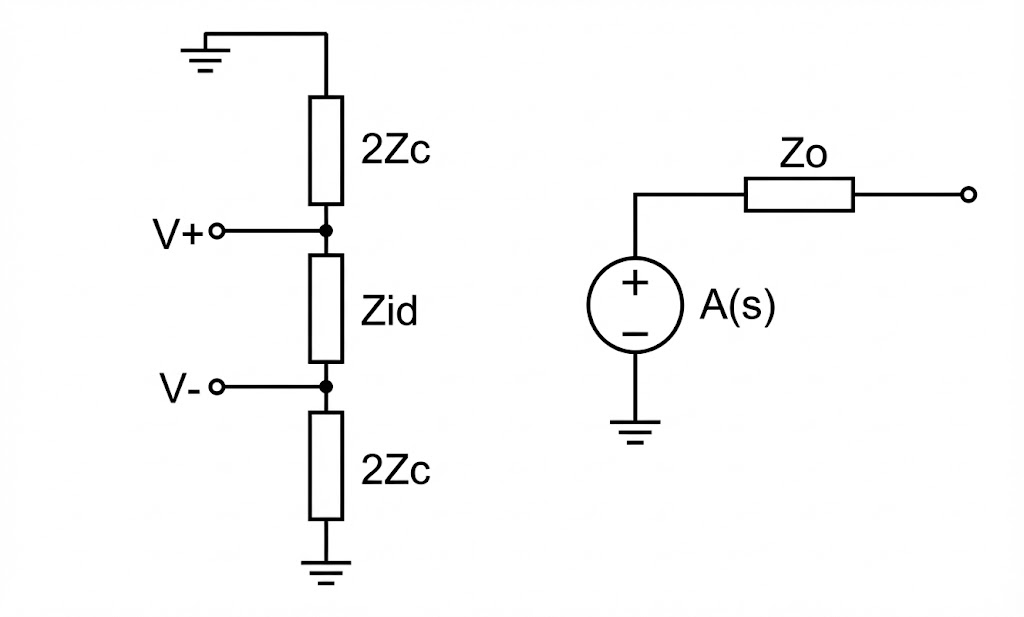
\includegraphics[width=0.5\linewidth]{Imagenes/1.1.png}
    \caption{Modelo del Amplificador  Operacional Real.}
    \label{fig:1.1}
\end{figure}
En general, interesa evaluar los efectos de primer orden que las características reales imponen sobre el comportamiento del amplificador. Si bien ciertos efectos críticos en una aplicación pueden resultar irrelevantes en otra, es posible asumir un modelo real simplificado, como se observa en la Figura~\ref{fig:1.2}a, que permita evaluar al menos los parámetros típicos; este análisis se abordará en el capítulo siguiente. Por otro lado, la Figura~\ref{fig:1.2}b presenta el modelo lineal de pequeña señal idealizado, el cual será utilizado en el desarrollo subsiguiente.
\begin{figure}[H]
    \centering
    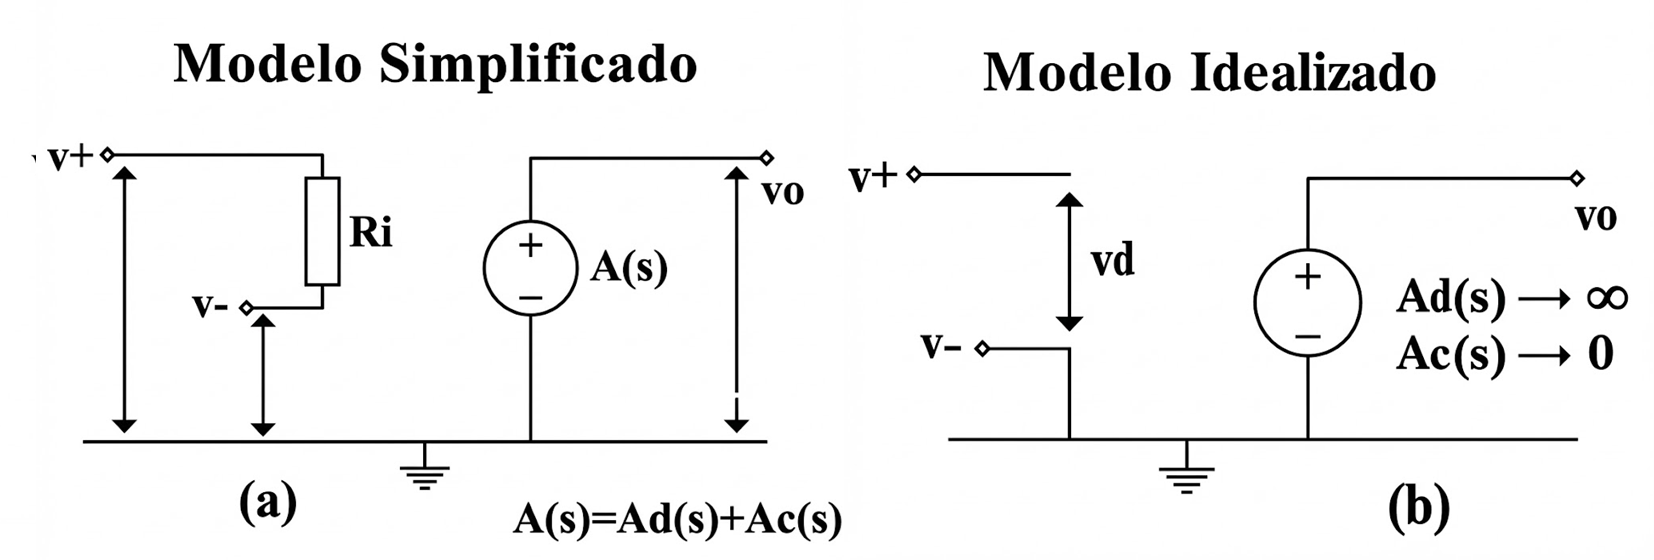
\includegraphics[width=0.85\linewidth]{Imagenes/1.2.png}
    \caption{Modelos del amplificador operacional}
    \label{fig:1.2}
\end{figure}
La figura ~\ref{fig:1.3}a muestra la estructura clásica de utilización del amplificador operacional, con la red de realimentación conectada. Esta es generalmente un cuadripolo pasivo (R-C) con un terminal común ~\ref{fig:1.3}b.
\begin{figure}[H]
    \centering
    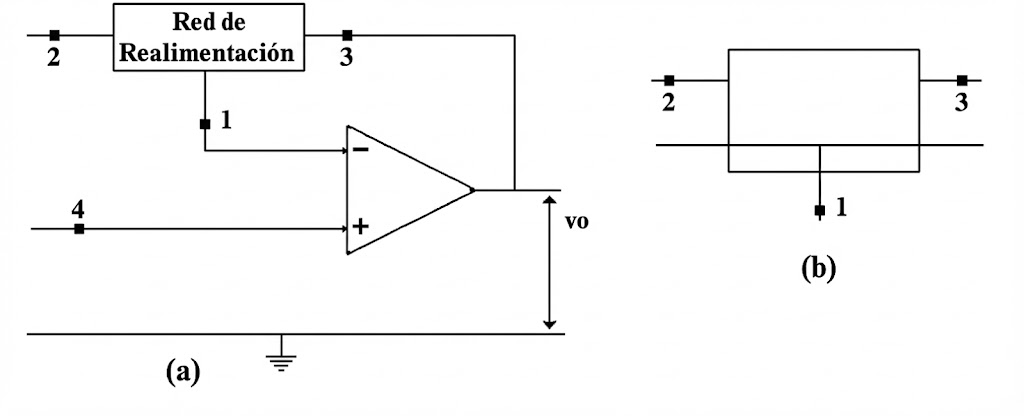
\includegraphics[width=0.85\linewidth]{Imagenes/1.3.png}
    \caption{Realimentación de un amplificador operacional}
    \label{fig:1.3}
\end{figure}
Dependiendo de si la señal excita el terminal (2), el (4) o ambos simultáneamente, se obtienen configuraciones inversoras, no inversoras o diferenciales, respectivamente. La utilización del modelo idealizado simplifica notablemente el análisis del circuito. Por ejemplo, considerar una impedancia de entrada infinita trae consigo las siguientes implicaciones:
\begin{figure}[H]
    \centering
    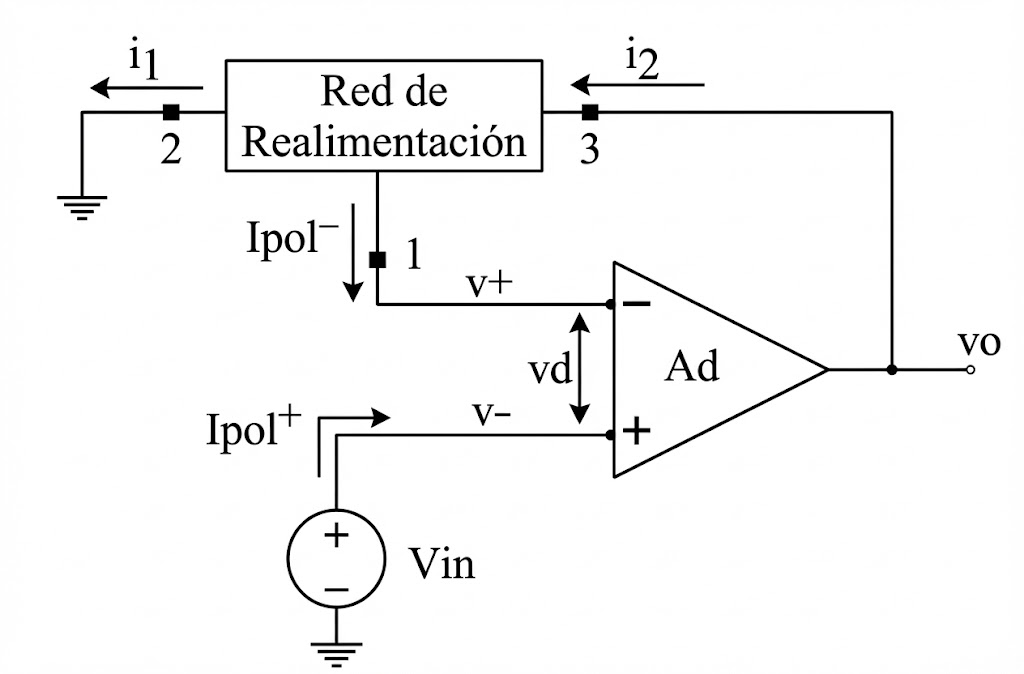
\includegraphics[width=0.5\linewidth]{Imagenes/1.4.png}
    \caption{Realimentación de un amplificador operacional}
    \label{fig:1.4}
\end{figure}
\vspace{-1.5em}
\begin{equation}
    Z_{id} \to \infty \implies I_{pol}^{-} = 0 \implies i_1 = i_2
    \label{eq:1.1}
\end{equation}

Además, si se considera una ganancia de modo diferencial infinita ($A_d \to \infty$), la única posibilidad de obtener una tensión de salida finita (según $v_o = A_d \cdot v_d$) es asegurando una tensión diferencial de entrada nula. Este hecho solo es posible retornando una fracción ($K$) de la señal de salida al terminal inversor con la fase apropiada (realimentación negativa), lo que conduce a:
\begin{equation}
    A_d \to \infty \implies v_d = (v^+ - v^-) \to 0 \implies v^+ = v^-
    \label{eq:1.2}
\end{equation}

La asunción hecha se traduce en un ``cortocircuito virtual'' a la entrada del amplificador. Si, sumadas a las conclusiones obtenidas, se consideran además la ganancia de modo común y la impedancia de salida nulas, la mayoría de las configuraciones básicas con A.O.\ se resuelven por simple inspección.
\subsection{Aplicaciones Lineales}
En la mayoría de las configuraciones, la red de realimentación es simplemente un divisor resistivo que ajusta la cantidad de realimentación introducida a la entrada inversora ($k \cdot v_o$), tal como muestra la Figura~\ref{fig:1.5} para los circuitos denominados inversor y no inversor. Para el primero de ellos, las conclusiones \eqref{eq:1.1} y \eqref{eq:1.2} llevan a:
\begin{equation}
    v^+ = v^- = 0 \quad \text{e} \quad i_2 = i_1 \implies \frac{v_o}{R_2} = -\frac{v_{in}}{R_1}
    \label{eq:1.3}
\end{equation}
\begin{figure}[H]
    \centering
    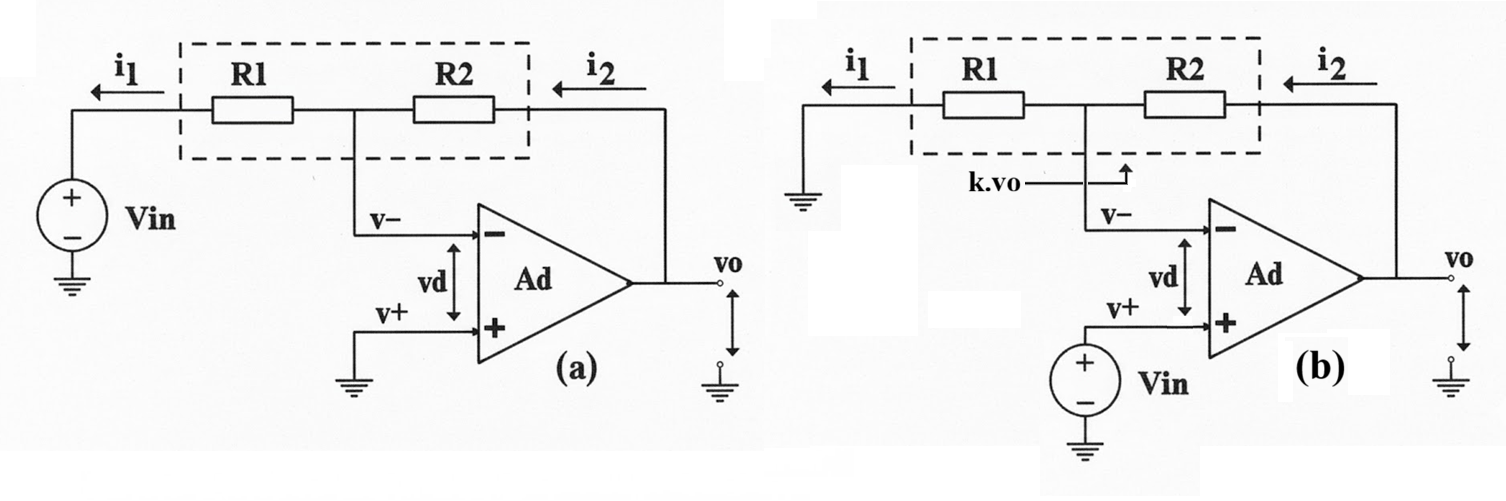
\includegraphics[width=0.95\linewidth]{Imagenes/1.5.png}
    \caption{Amplificador inversor}
    \label{fig:1.5}
\end{figure}
Luego:
\begin{equation}
    A_{vfi} = \frac{v_o}{v_{in}} = -\frac{R_2}{R_1} \qquad A_{vfi} = \text{Ganancia de tensión ideal.}
    \label{eq:1.4}
\end{equation}

Teniendo en cuenta que:
\begin{equation}
    K = \frac{R_1}{R_1 + R_2} \implies A_{vfi} = \left( 1 - \frac{1}{K} \right)
    \label{eq:1.5}
\end{equation}

De igual manera en el circuito no inversor:
\begin{equation}
    i_1 = i_2 \implies \frac{v_o - v^+}{R_2} = \frac{v^-}{R_1}
    \label{eq:1.6}
\end{equation}

\begin{equation}
    v^+ = v^- = v_{in} \implies A_{vfi} = \frac{R_1 + R_2}{R_1} = 1 + \frac{R_2}{R_1} = \frac{1}{K}
    \label{eq:1.7}
\end{equation}
La figura ~\ref{fig:1.6} muestra una configuración que esta excitada en los dos terminales en la que se demuestra que la tensión de salida es proporcional al modo diferencial de las señales de entrada.
\begin{figure}[H]
    \centering
    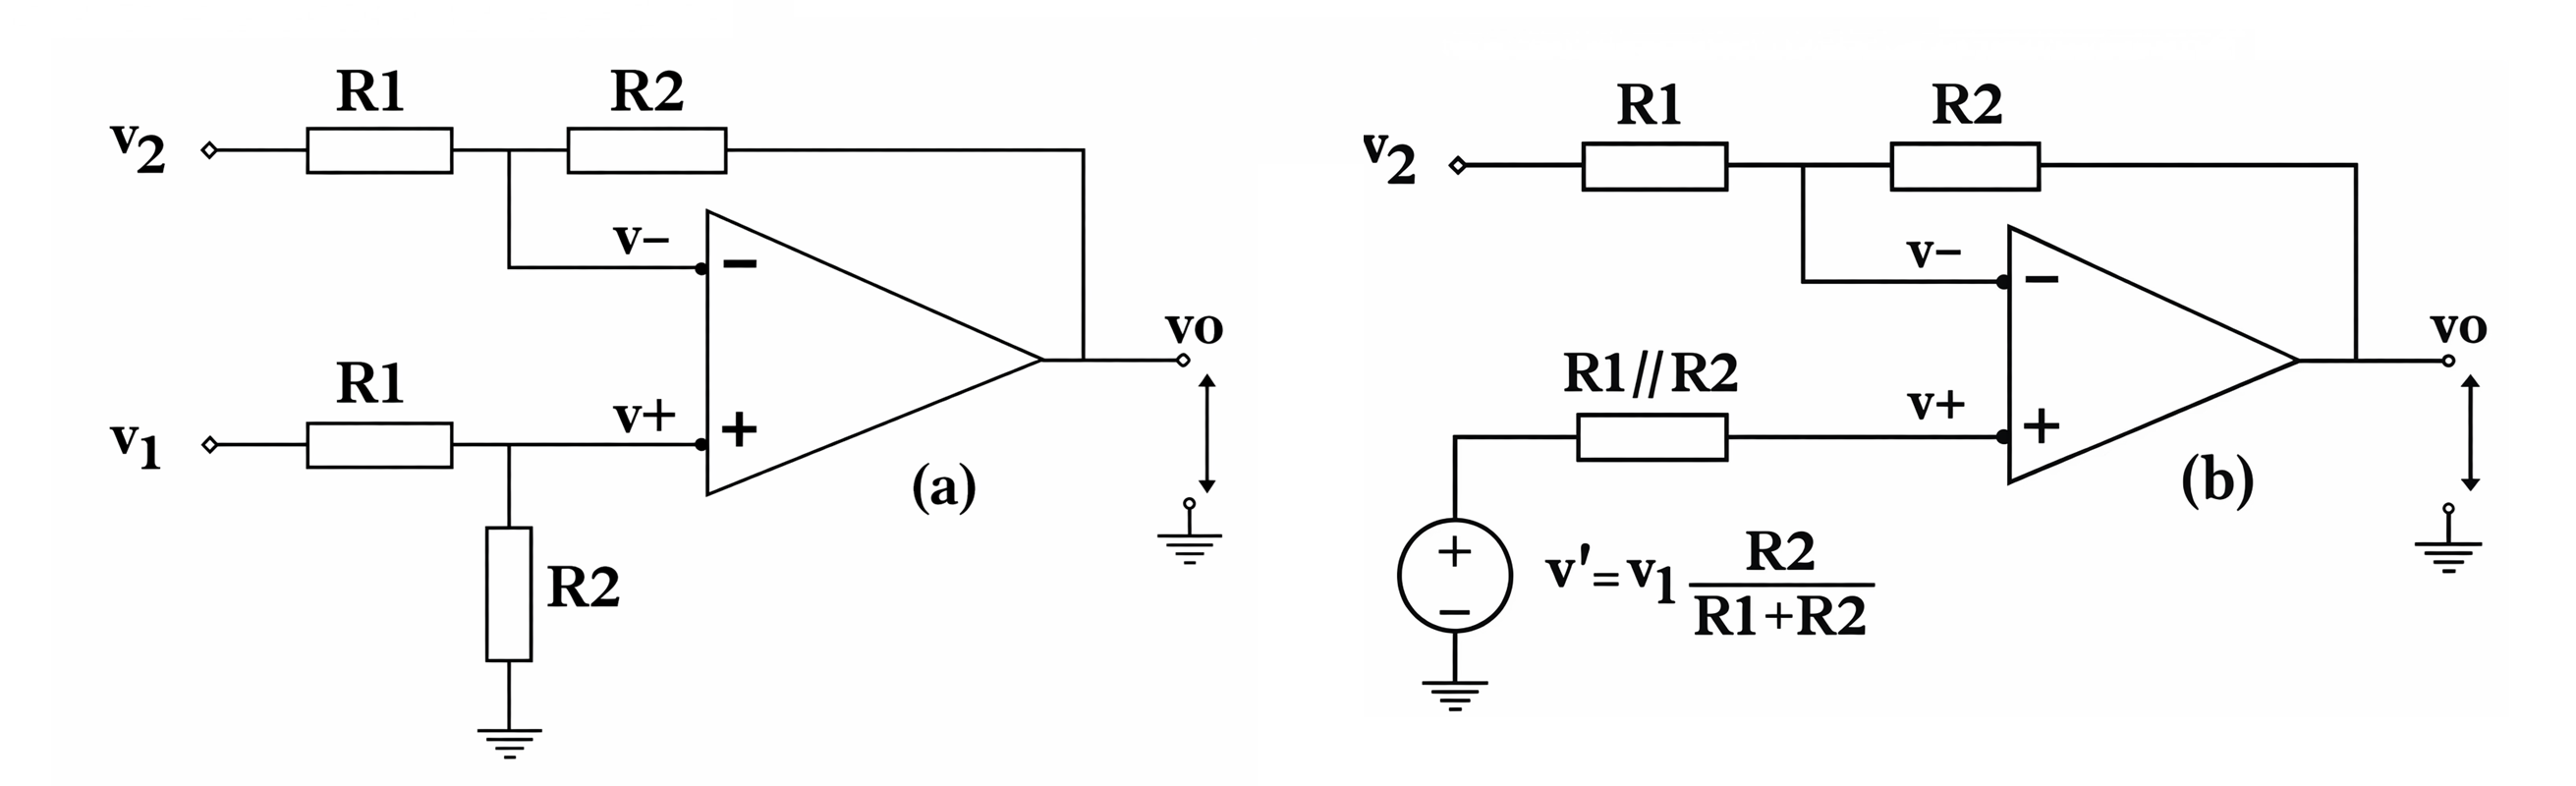
\includegraphics[width=0.95\linewidth]{Imagenes/1.6.png}
    \caption{Modo diferencial}
    \label{fig:1.6}
\end{figure}
En efecto, utilizando superposición queda una configuración inversora al pasivar $V_1$, y no inversora al hacerlo con $V_2$; luego, utilizando las conclusiones anteriores \eqref{eq:1.4} y \eqref{eq:1.7} se obtiene:

\[
v_0 = \left[ -\frac{R_2}{R_1} \cdot v_2 \right]_{V_1 = 0} + \left[ v' \cdot \left( 1 + \frac{R_2}{R_1} \right) \right]_{V_2 = 0}
\]

La que luego de operarla lleva a: 
\begin{equation}
    v_0 = (v_1 - v_2) \frac{R_2}{R_1} \implies A_{vfi} = \frac{v_0}{v_1 - v_2} = \frac{R_2}{R_1}
    \label{eq:1.8}
\end{equation}
\vspace{1em} % Espacio opcional antes del bloque
\hrule height 1.5pt % Línea gruesa superior
\vspace{2pt}
\noindent {\large \textbf{Problema.}}
\vspace{4pt}
\hrule height 1pt % Línea inferior
\vspace{1.5em}

Utilizando superposición, demuestre que la tensión de salida del diferencial de la figura es:

\[
v_o = (v_2 - v_1) + v_X
\]
\vspace{-2em}
\begin{figure}[H]
    \centering
    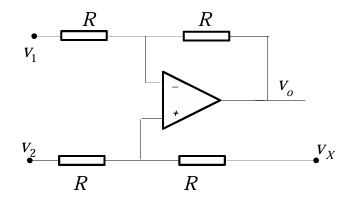
\includegraphics[width=0.5\linewidth]{Imagenes/1.E.png}
\end{figure}
\hrule height 1.5pt % Línea gruesa superior
\vspace{2pt}
Para generar funciones de filtros (pasa bajos, pasa banda, etc.), la red de realimentación está compuesta por resistores y capacitores. Aquellos circuitos que realizan funciones de primer grado (un polo o un cero real) también pueden analizarse por simple inspección. Por ejemplo, el que muestra la Figura~\ref{fig:1.7} es un filtro pasa alto inversor de grado uno.
\begin{figure}[H]
    \centering
    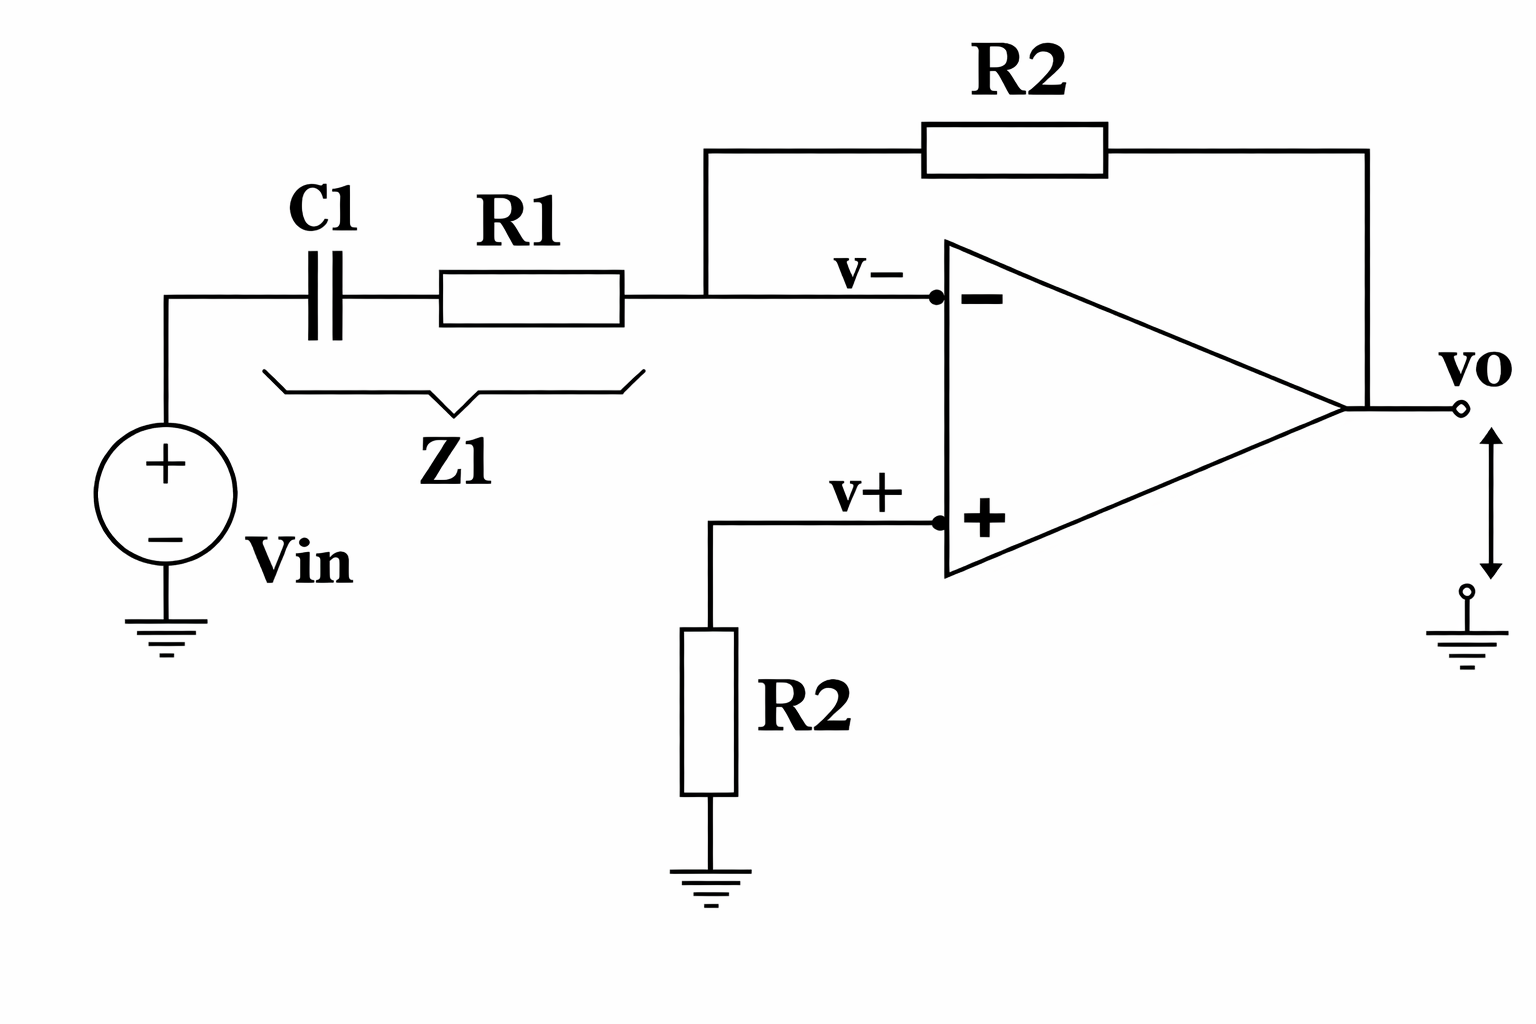
\includegraphics[width=0.5\linewidth]{Imagenes/1.7.png}
    \caption{Filtro pasa alto}
    \label{fig:1.7}
\end{figure}
Tratándose de una configuración inversora, su ganancia es:

\begin{align}
    A_{vf}(s) &= -\frac{R_2}{Z_1} = -\frac{R_2}{R_1 + \dfrac{1}{s \cdot C_1}} = -\frac{s \cdot C_1 \cdot R_2}{1 + s \cdot C_1 \cdot R_1} \notag \\
    \notag \\
    A_{vf}(s) &= -\frac{R_2}{R_1} \cdot \frac{s}{s + a} = -A_{vf}(\infty) \cdot \frac{s}{s + a} \label{eq:1.9} \\
    A_{vf}(\infty) &= \frac{R_2}{R_1} \to \text{(Asíntota de alta frecuencia)} \notag
\end{align}

Es interesante comparar la respuesta del circuito activo de la Figura~\ref{fig:1.7} con la de un filtro pasivo equivalente. El circuito pasivo en cuestión se muestra en la Figura~\ref{fig:1.8}, y su F.T.\ es la siguiente:

\begin{nointerlineskip}
\begin{minipage}{0.5\textwidth}
    \begin{align*}
        A_v(s) &= \frac{v_0}{v_{in}} = \frac{s}{s + \dfrac{1}{C_1 \cdot R_1}} = \frac{s}{s + a} \\
        A_{vf}(\infty) &= 1
    \end{align*}
\end{minipage}
\begin{minipage}{0.5\textwidth}
    \centering
    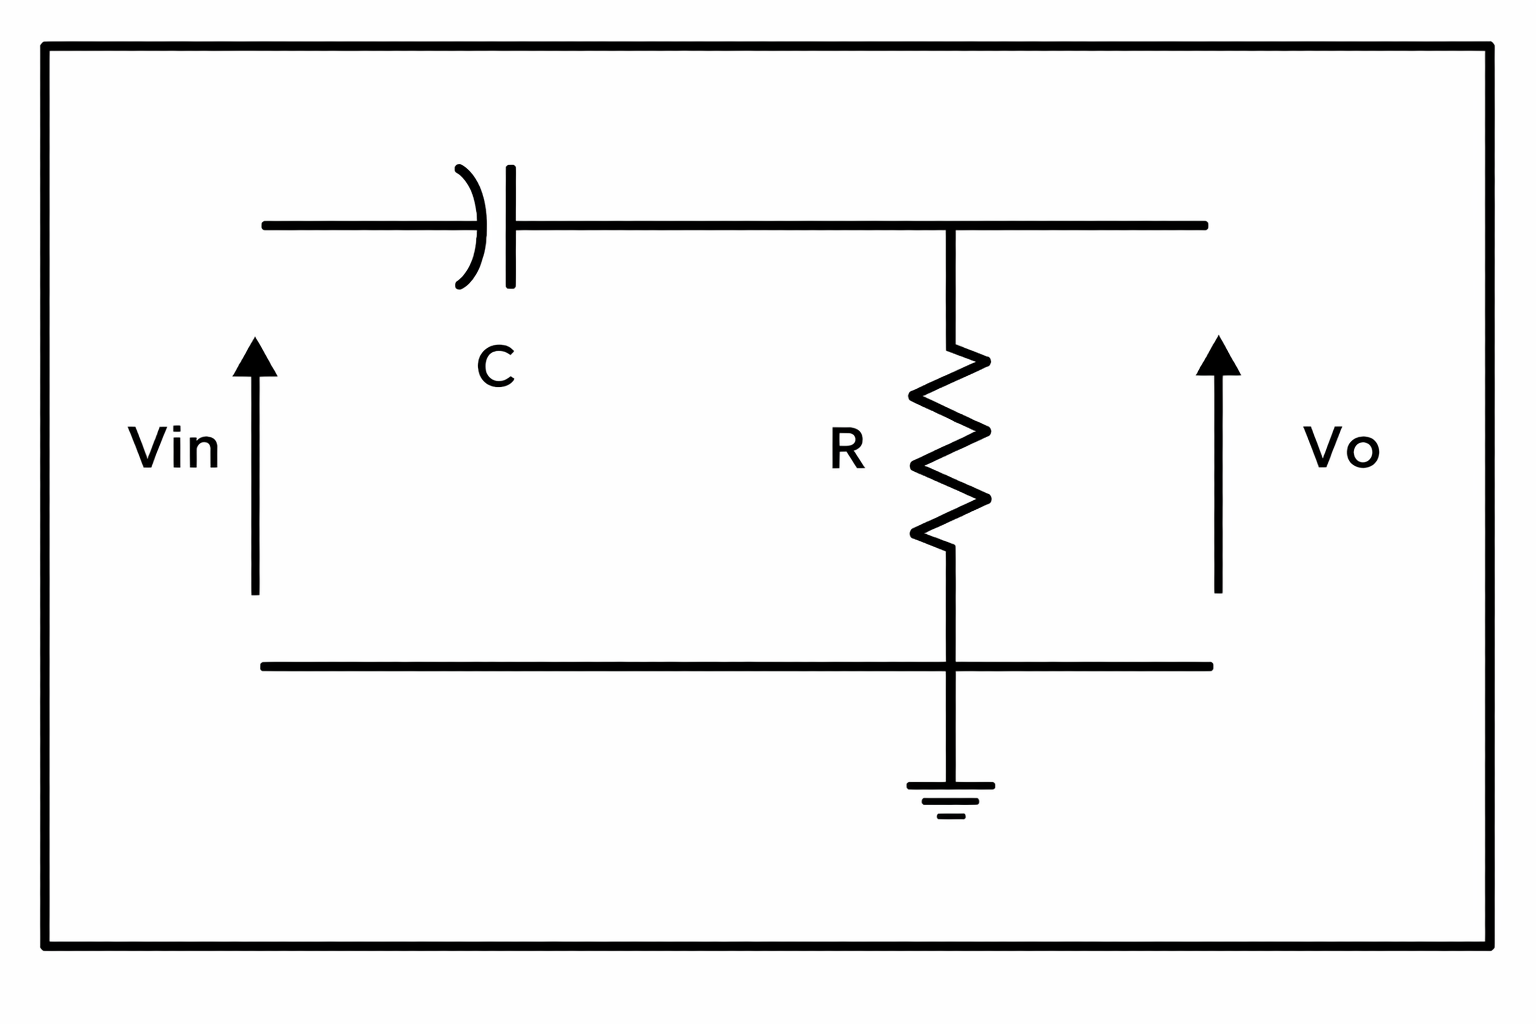
\includegraphics[width=0.7\linewidth]{Imagenes/1.8.png}
    \captionof{figure}{Filtro RC pasivo}
    \label{fig:1.8}
\end{minipage}
\end{nointerlineskip}

Comparando las funciones de transferencia anteriores, se aprecia la ganancia adicional que aporta el filtro activo en la banda de paso ($A_{vf}(\infty) = R_2/R_1 > 1$), frente a la máxima que puede otorgar su homónimo pasivo, que es la unidad. En el diagrama de la Figura~\ref{fig:1.9} se aprecian ambas respuestas en módulo.
\begin{figure}[H]
    \centering
    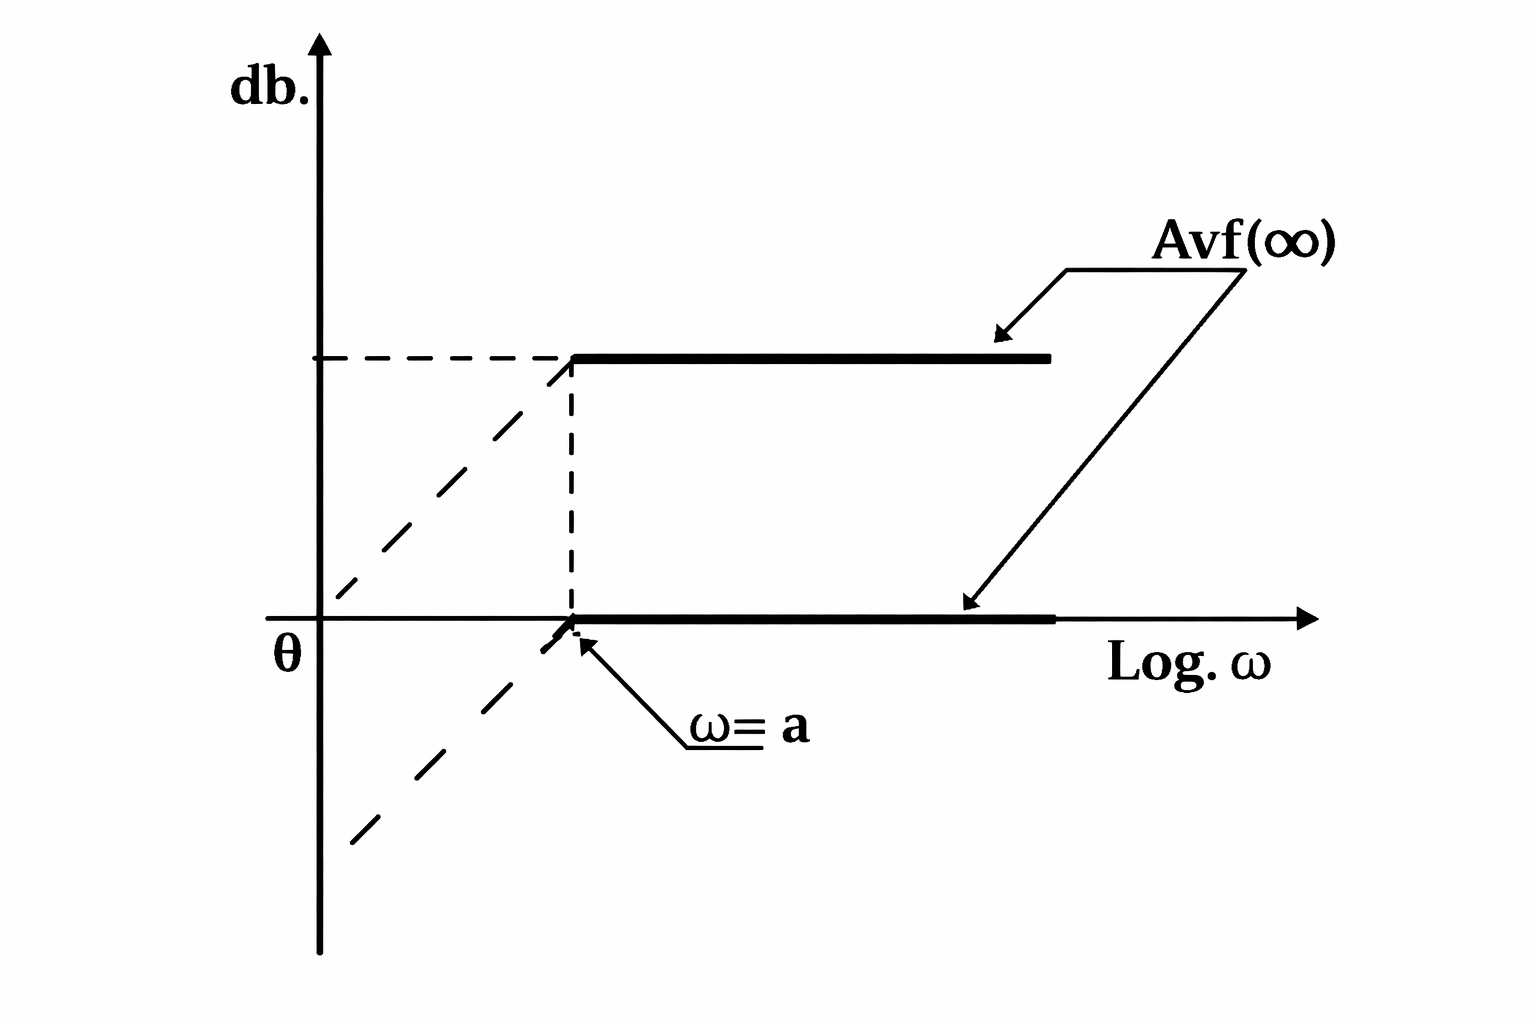
\includegraphics[width=0.5\linewidth]{Imagenes/1.9.png}
    \caption{Respuesta de bode del filtro}
    \label{fig:1.9}
\end{figure}
\subsubsection{Fuentes de corriente}
La Figura~\ref{fig:1.10} muestra una configuración amplificadora que tiene un lazo de realimentación negativa ($R_2$) y otro positivo ($R_1$). Tiene la característica de presentar impedancia negativa en determinadas secciones del mismo (NIC). Esta propiedad se deduce para la impedancia vista hacia la entrada no inversora ($Z^+$). En efecto, teniendo en cuenta que en condiciones ideales las tensiones en ambas resistencias de realimentación son iguales, se obtiene:

\begin{equation}
    \text{Si } v^- = v^+ \implies I_1 \cdot R_1 = -I_2 \cdot R_2 \implies I_2 = I_3 = -\left( \frac{R_1}{R_2} \right) \cdot I_1
    \label{eq:1.10}
\end{equation}

Luego:
\begin{equation}
    Z^+ \cdot I_1 = R_3 \cdot I_3 \implies Z^+ = \left( \frac{I_3}{I_1} \right) \cdot R_3 = -\left( \frac{R_1}{R_2} \right) \cdot R_3
    \label{eq:1.11}
\end{equation}

Intercambiando en la Figura~\ref{fig:1.10} la excitación con $R_3$, se obtiene para la impedancia vista desde la inversora una expresión equivalente:

\begin{equation*}
    Z^- = -\left( \frac{R_2}{R_1} \right) \cdot R_3
\end{equation*}

Ambas muestran una resistencia negativa cuyo valor es una combinación lineal de las conectadas.

Debido a que en el circuito hay realimentación de ambos signos, puede hacerse inestable en el caso de que la neta sea positiva. Esto ocurriría, por ejemplo, en el esquema de la Figura~\ref{fig:1.10} si el nodo no inversor es excitado por una fuente de corriente ideal, debido a que:

\[
K^+ = 1 > K^- = \frac{R_3}{(R_2 + R_3)}
\]

Para revertir esta situación, es necesario que la fuente de excitación tenga una resistencia asociada ($R_4$) de un valor máximo dado por la siguiente relación:

\begin{equation}
    R_4 \le R_3 \cdot \frac{R_1}{R_2}
    \label{eq:1.12}
\end{equation}
\begin{figure}[H]
    \centering
    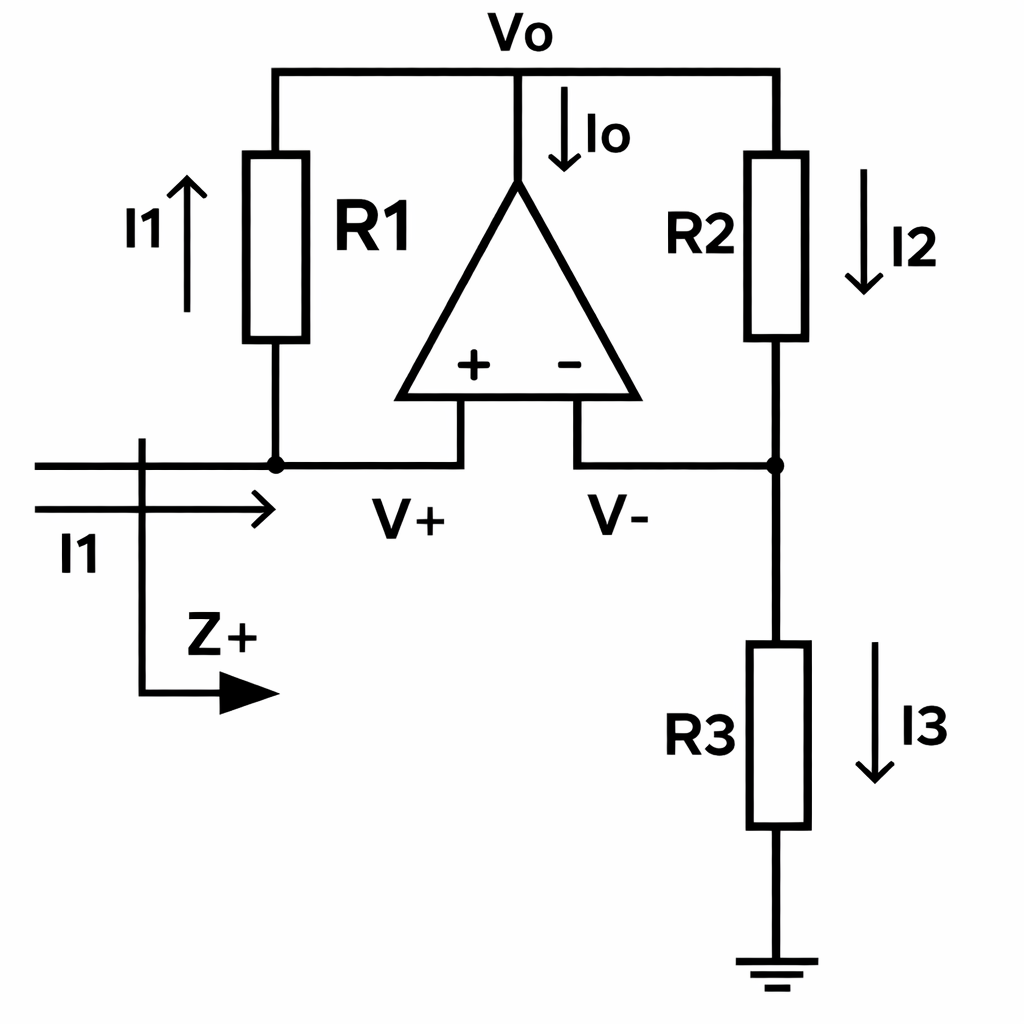
\includegraphics[width=0.5\linewidth]{Imagenes/1.10.png}
    \caption{Conversor a  Inmitancia  Negativa }
    \label{fig:1.10}
\end{figure}
Esta propiedad de convertir una inmitancia real en negativa posee variadas aplicaciones; por ejemplo, permite cancelar el efecto de una resistencia asociada externamente al terminal en cuestión. La Figura~\ref{fig:1.11}a muestra una aplicación que consiste en una fuente de corriente ($I_L$) de impedancia interna infinita controlada por tensión ($V_{in}$), circuito conocido como la bomba de corriente de Howland (desarrollada por B. Howland, M.I.T.).
\begin{figure}[H]
    \centering
    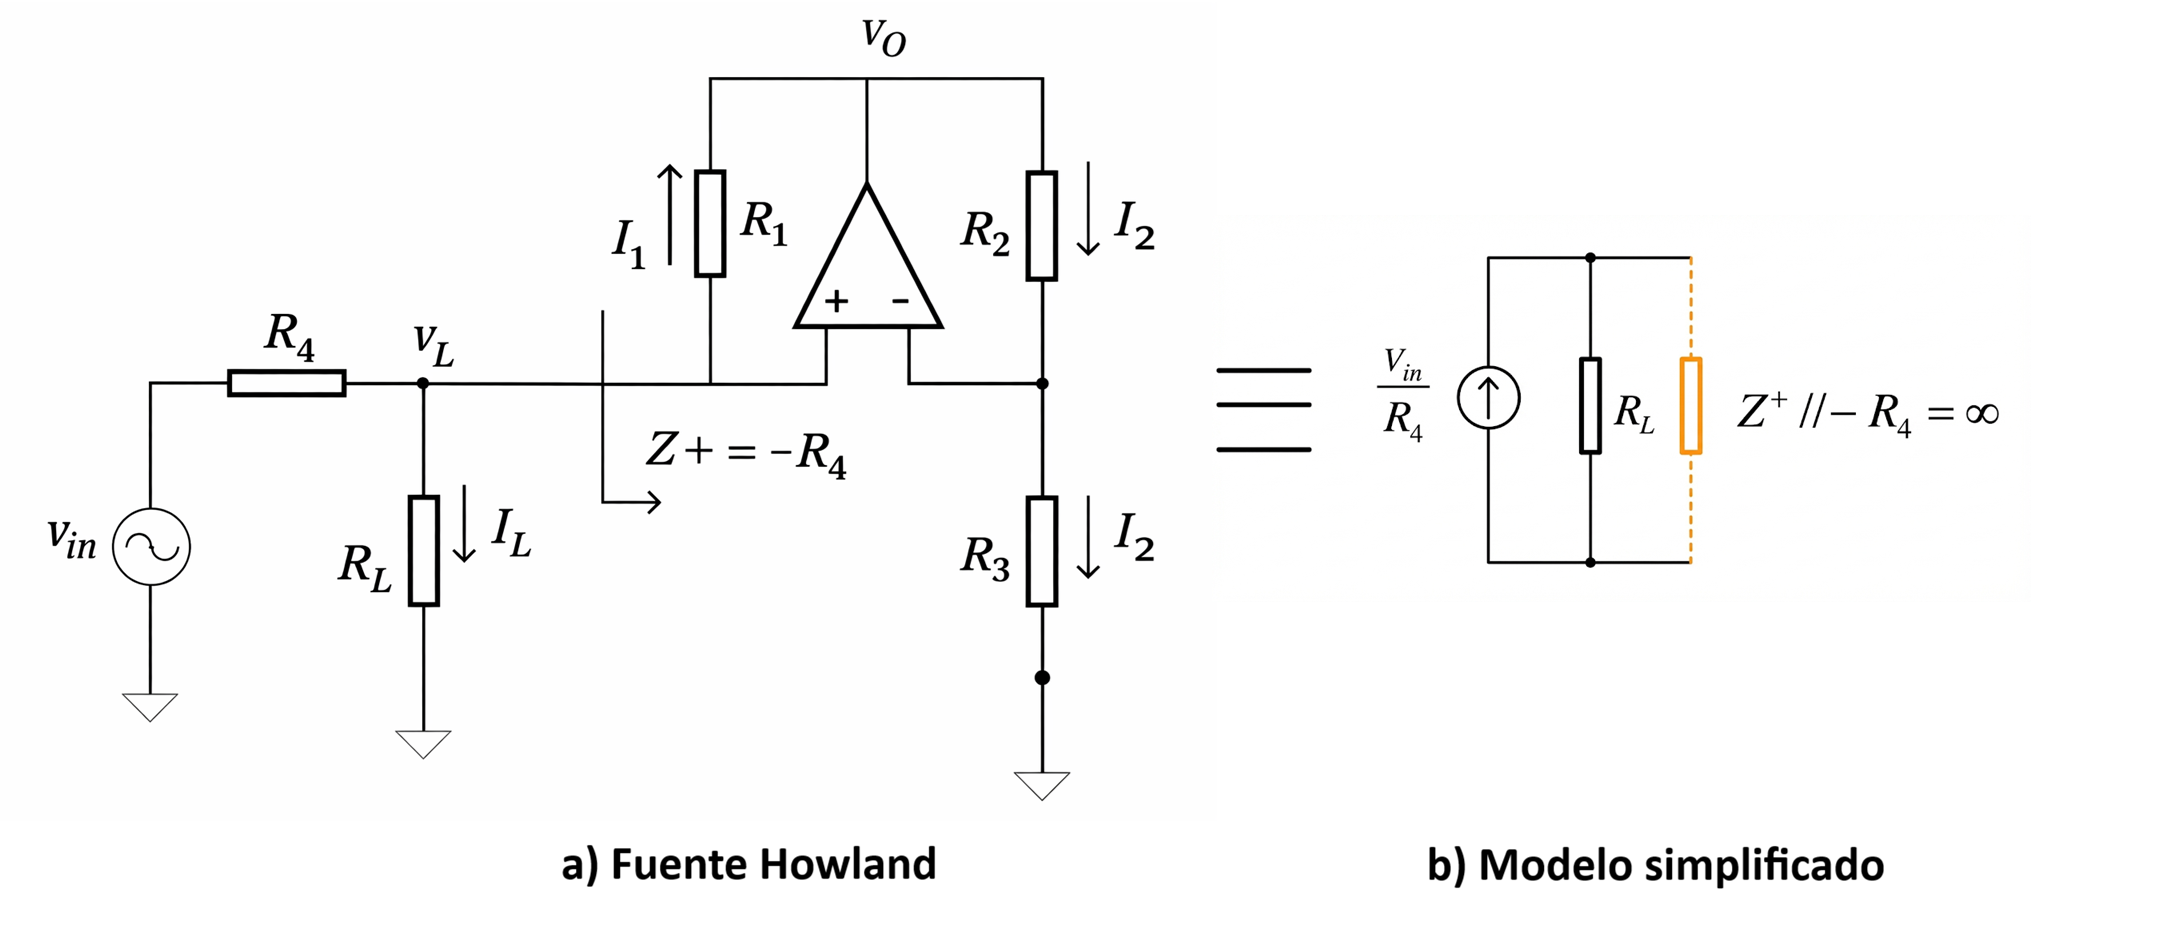
\includegraphics[width=0.95\linewidth]{Imagenes/1.11.png}
    \caption{Simplificación de la fuente Howland}
    \label{fig:1.11}
\end{figure}
Del circuito reducido \eqref{eq:1.11}b, se deduce que si se ajustan adecuadamente los valores dados en \eqref{eq:1.11} se cumple la siguiente relación:

\[
Z^+ = -R_4
\]

Resultando la impedancia vista por la carga de valor infinito, en consecuencia es:
\begin{equation}
    I_L = \frac{V_{in}}{R_4}
    \label{eq:1.13}
\end{equation}

Para ajustar el diseño se deben tener en cuenta las siguientes consideraciones. Por ejemplo, debido a que la tensión de salida del amplificador resulta proporcional a la resistencia de carga \eqref{eq:1.14} y teniendo presente que aquella es inferior a la de alimentación del operacional, la ganancia no inversora que muestra la ecuación de referencia debe bajar, en la medida que aumenta el rango de carga ($R_L$). Esto obliga a reducir $R_2/R_3$ para no exceder $V_{omax}$.

\begin{equation}
    v_o = V^+ \cdot \left( 1 + \frac{R_2}{R_3} \right) = R_L \cdot I_L \cdot \left( 1 + \frac{R_2}{R_3} \right) = \text{Cte.} \cdot R_L \implies R_{Lmax} = \frac{V_{omax}}{\text{Cte.}}
    \label{eq:1.14}
\end{equation}

En consecuencia, un criterio de diseño sería: conocida $V_{omax}$ y la tensión a generar, $V_{Lmax}$, se puede definir la ganancia no inversora máxima y luego con \eqref{eq:1.11} calcular $R_1$.

\[
\frac{V_{omax}}{I_L \cdot R_{Lmax}} \le 1 + \frac{R_2}{R_3} \quad \to \quad R_1 \le R_4 \cdot \frac{R_2}{R_3} \qquad \text{\small (ATENCIÓN: POSIBLE ERROR!)}
\]

Debido a que en un caso de aplicación práctica se deben conectar resistencias comerciales, existirán desviaciones en las relaciones arriba asumidas. En efecto, si se evalúa la impedancia vista por la resistencia de carga en el circuito de la Fig.~1.11b, admitiendo una desviación $\Delta\alpha$ entre los parámetros de ajuste de las relaciones anteriores, se obtiene utilizando \eqref{eq:1.11}:

\begin{equation}
    Z_O = R_4 \, // \, Z^+ = \frac{(1 + \Delta\alpha) \cdot R_4}{\Delta\alpha}
    \label{eq:1.15}
\end{equation}

La anterior muestra que la impedancia interna de la fuente de corriente deja de ser infinita a menos que se corrija la desviación modificando la resistencia adecuada elegida entre las cuatro involucradas.
El esquema (a) de la Figura~\ref{fig:1.12} muestra una fuente de corriente controlada por el modo diferencial de entrada. Dicho esquema puede interpretarse según (b), con el lazo de realimentación positiva abierto y considerando que la impedancia vista desde la sección indicada es mucho mayor que la de carga.
\begin{figure}[H]
    \centering
    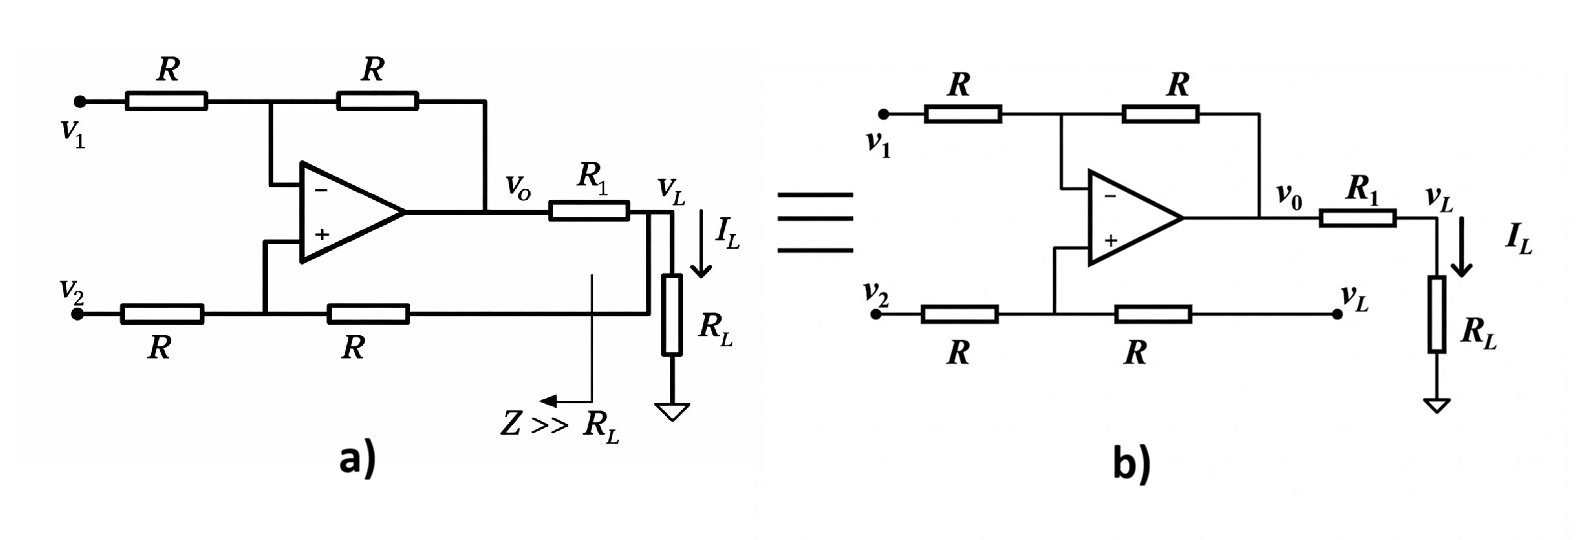
\includegraphics[width=0.85\linewidth]{Imagenes/1.12.png}
    \caption{Fuente de corriente en modo diferencial.}
    \label{fig:1.12}
\end{figure}
Del esquema (b), teniendo presente la conclusión del circuito presentado en E.1, se deducen las siguientes relaciones:

\[
I_L = \frac{v_o - v_L}{R_1} \quad \text{y} \quad v_L = v_o \frac{R_L}{R_1 + R_L} \quad \text{además} \quad v_o = (v_2 - v_1) + v_L
\]

Eliminando $v_o$ de las anteriores se obtiene finalmente:
\begin{equation}
    I_L = \frac{v_2 - v_1}{R_1} = \frac{V_d}{R_1}
\end{equation}

La carga máxima admitida, ($R_{Lmax}$), en operación lineal, de igual manera que en el caso anterior está relacionada con la excursión máxima permitida del AO. En efecto, conocido el modo diferencial máximo aplicado y la corriente de carga requerida, se cumple:

\begin{equation}
    v_{omax} = I_L (R_1 + R_{Lmax})
\end{equation}

Otro parámetro importante del comportamiento de la fuente de corriente es su impedancia interna que puede ser evaluada en el esquema equivalente dado a continuación. En este y en términos ideales se explicita únicamente el lazo que realimenta positivamente al amplificador no inversor de ganancia 2.
\begin{figure}[H]
    \centering
    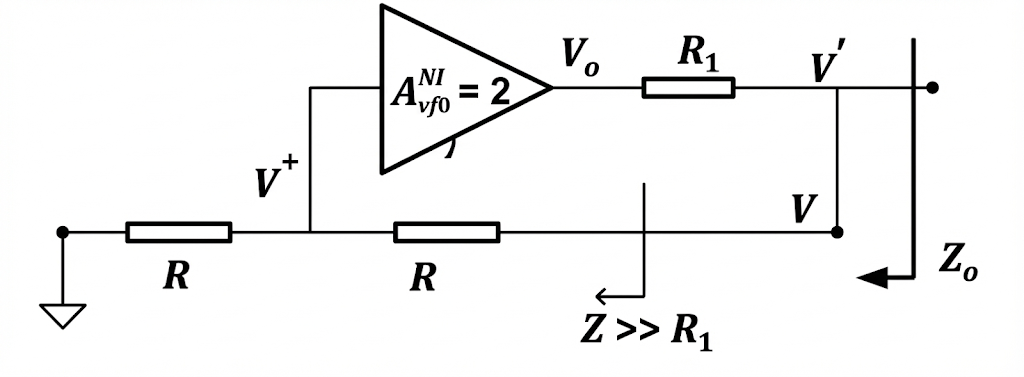
\includegraphics[width=0.5\linewidth]{Imagenes/1.13.png}
    \caption{Impedancia interna}
    \label{fig:1.13}
\end{figure}
Abriendo el lazo en la línea de puntos se deduce, a partir de la expresión de Blackman:

\begin{equation}
    Z_O = R \cdot \frac{1 - T_{CC}}{1 - T_{CA}} \qquad R = \text{Impedancia de sistema muerto, } (v = 0) = R_1
\end{equation}

\[
T_{CC} = \frac{v'}{v} = 0 \quad \text{Debido a que no hay retorno de lazo en la sección de interés } (v' = 0).
\]

En cambio, a sección abierta resulta:

\begin{equation}
    T_{CA} = \frac{v'}{v} = \frac{v^+}{v} \cdot \frac{v'}{v^+} = \frac{1}{2} A_{vfi}^{NI} = +1 \qquad \text{Luego} \qquad Z_0 = \frac{R_1}{1 - 1} = \infty
\end{equation}

Obviamente resulta infinita idealizando el AO; no obstante, en el caso real es finita y de valor muy elevado.
\subsection{Aplicaciones no lineales}
\subsubsection{Amplificador logarítmico}
Obviamente, cuando en la red de realimentación intervienen elementos no lineales activos o pasivos, las relaciones de transferencia resultan no lineales (la salida no es una réplica escalada de la entrada). En términos generales (caso lineal y no lineal), se puede demostrar que cuando en el lazo de realimentación negativa se introduce un bloque funcional definido como $A_f = I_o / V_o$ (Figura~\ref{fig:1.14}), la salida del amplificador realimentado realiza la función inversa, siempre que la función realimentada ($A_f$) no tenga discontinuidades en el rango de operación.
\begin{figure}[H]
    \centering
    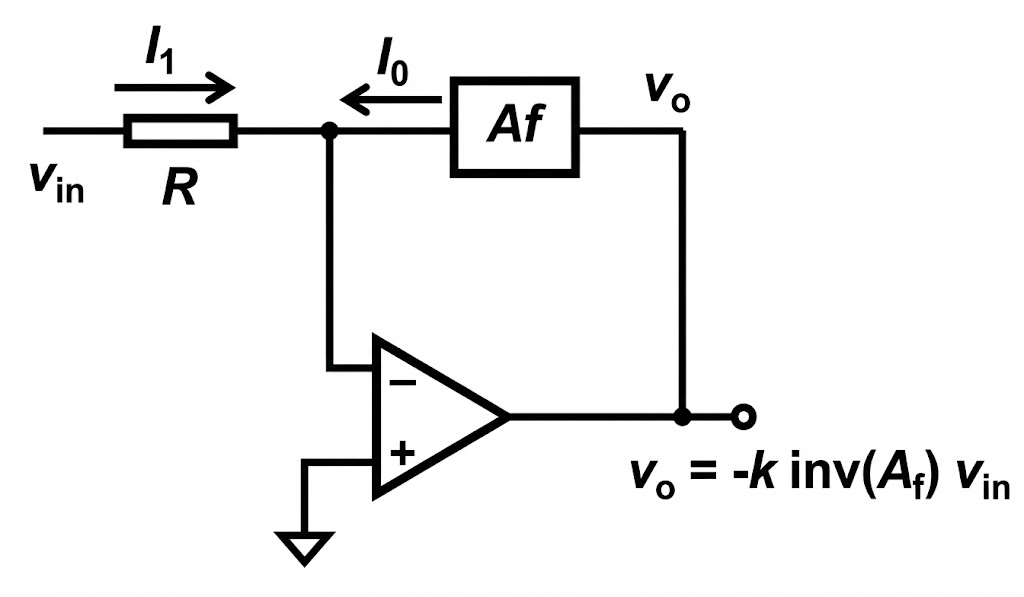
\includegraphics[width=0.5\linewidth]{Imagenes/1.14.png}
    \caption{Amplificador logaritmico}
    \label{fig:1.14}
\end{figure}
Dos casos no lineales típicos son el amplificador logarítmico y los rectificadores de precisión. El primero de ellos se muestra en la Figura~\ref{fig:1.15}, en la cual la tensión de salida se corresponde con la de una junta P-N directamente polarizada (base-emisor). Siendo la relación tensión-corriente exponencial ($I_C \approx I_{S} \cdot e^{k \cdot V_{be}}$), la tensión de salida debería tener una relación inversa (logarítmica) con la corriente inyectada al nudo inversor.
\begin{figure}[H]
    \centering
    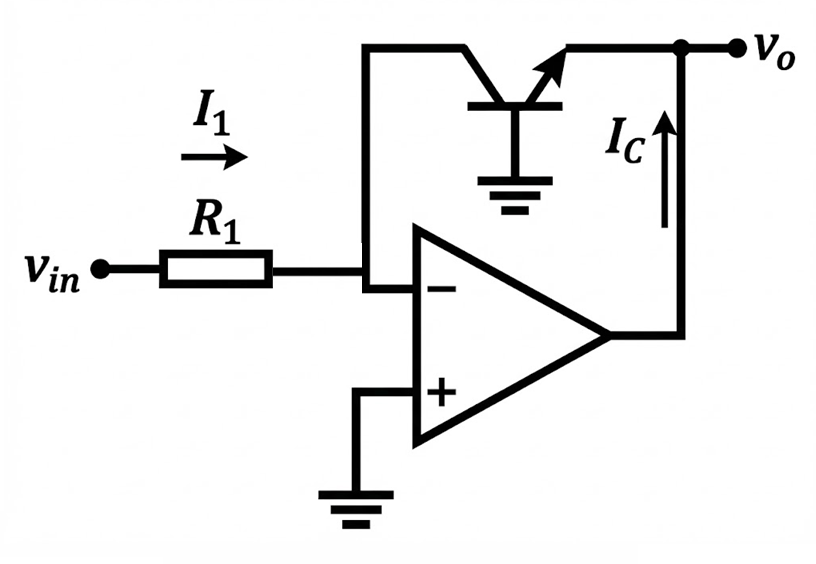
\includegraphics[width=0.5\linewidth]{Imagenes/1.15.png}
    \caption{Modelo de Ebbers-Moll}
    \label{fig:1.15}
\end{figure}
En efecto, el modelo de Ebers-Moll describe el comportamiento de la corriente de colector de un transistor bipolar en términos de la ecuación diódica de Shockley, según la siguiente expresión:

\begin{equation}
    I_C = \alpha_F \cdot I_{ES} \cdot (e^{\frac{V_{BE}}{V_t}} - 1) - I_{CS} \cdot (e^{\frac{V_{BC}}{V_t}} - 1)
    \label{eq:1.16}
\end{equation}

Donde: $V_t = \dfrac{K \cdot T}{q} \cong 26 \text{ mV}$ (T = 300 °K)

Si en el circuito de la Figura 1.13 se cumple que: $A_d \to \infty \implies v_d \to 0 \implies V_{CB} = 0$, la anterior resulta:

\begin{equation}
    I_C = \alpha_F \cdot I_{ES} \cdot (e^{\frac{V_{BE}}{V_t}} - 1) = I_{C0} \cdot (e^{\frac{V_{BE}}{V_t}} - 1)
    \label{eq:1.17}
\end{equation}

$I_{C0} = \text{corriente de saturación inversa de la junta base emisor.}$

Si la junta base emisor es polarizada directamente con tensiones $V_{BE} > 4V_t \cong 100 \text{ mV}$, se puede tomar la corriente de colector en forma simplificada:

\begin{equation}
    I_C \cong I_{C0} \cdot (e^{\frac{V_{BE}}{V_t}})
    \label{eq:1.18}
\end{equation}

Los transistores de señal siguen muy ajustadamente esta ley dentro de un rango de valores de corrientes de colector del orden de 6 décadas (ej: 100 pA $\to$ 100 $\mu$A).

Finalmente, combinando la anterior con las relaciones de corriente del esquema de referencia, se obtiene la siguiente relación logarítmica:

\begin{equation}
    I_1 = \frac{V_{in}}{R_1} = I_C \implies V_o = -V_{BE} = -V_t \cdot \ln \left( \frac{V_{in}}{R_1 \cdot I_{C0}} \right)
    \label{eq:1.19}
\end{equation}

Generalmente, esta salida es invertida por un amplificador de ganancia unitaria.
Es importante analizar los órdenes de magnitud involucrados en la expresión anterior. Por ejemplo, debido a que el valor máximo de la señal de entrada generalmente no supera los diez voltios y el mínimo está limitado por la tensión de offset del amplificador (del orden de los milivolt), el rango dinámico típico de la señal de entrada es de 4 décadas (80 dB). Esto resulta aproximadamente en una excursión de la tensión de salida de:

\[
\Delta V_o \cong 26 \text{ mV} \cdot \ln(10000) = 240 \text{ mV}
\]

Este efecto de compresión de la señal de entrada visto desde la salida es una de las características relevantes del amplificador y es utilizada ampliamente en compresión de datos de señales de video.

Debido a que la expresión \eqref{eq:1.18} es válida siempre y cuando la junta base-emisor tenga polarización directa, la tensión de entrada debe ser siempre positiva, $V_{in} \ge 0$ (Amplificador Logarítmico de un cuadrante).

La relación de transferencia encontrada, vista en un gráfico de escala semi-logarítmica (en base 10), es una línea recta (Fig. 1.16), cuya pendiente es de aproximadamente 60 mV por cada década de variación de la magnitud de la señal de entrada.

\begin{equation}
    \Delta V_o = V_t \cdot \frac{\log(\Delta V_{in})}{\log(e)} = \frac{V_t}{\log(e)} \cdot \log(\Delta V_{in}) \cong 60 \text{ mV} \cdot \log(\Delta V_{in})
\end{equation}
\begin{figure}[H]
    \centering
    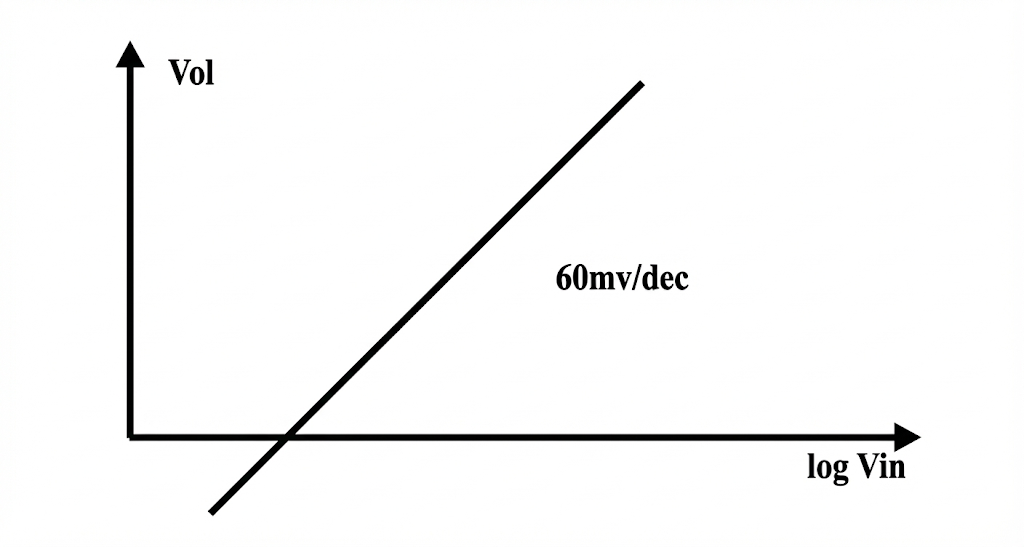
\includegraphics[width=0.5\linewidth]{Imagenes/1.16.png}
    \caption{Relación de transferencia}
    \label{fig:1.16}
\end{figure}
La abscisa al origen de dicha recta es:

\begin{equation}
    V_{in} = I_{C0} \cdot R_1
\end{equation}

La dependencia directa de la pendiente de la relación de transferencia con la temperatura absoluta a través del parámetro $V_t$ y la deriva del cruce por cero debido a la corriente de saturación inversa ($I_{C0}$) ---la cual aproximadamente se duplica cada 10 °C--- se transforman en el talón de Aquiles de esta configuración. 

Ambos problemas tienen variadas soluciones circuitales; una de ellas se muestra en el diagrama en bloques de la Figura~\ref{fig:1.17}, en la que un segundo amplificador logarítmico, idéntico a su homólogo y con ambos transistores térmicamente apareados, es excitado por una tensión muy estable ($V_{ref}$). Su salida ataca la entrada inversora de un amplificador diferencial de ganancia $A$, tal que la relación de transferencia total resulta:

\begin{equation}
    V_o = A \cdot V_t \cdot \ln \left( \frac{V_{in}}{V_{ref}} \right) = A \cdot V_t \cdot \frac{\log \left( \frac{V_{in}}{V_{ref}} \right)}{\log(e)}
    \label{eq:1.20}
\end{equation}

\begin{figure}[H]
    \centering
    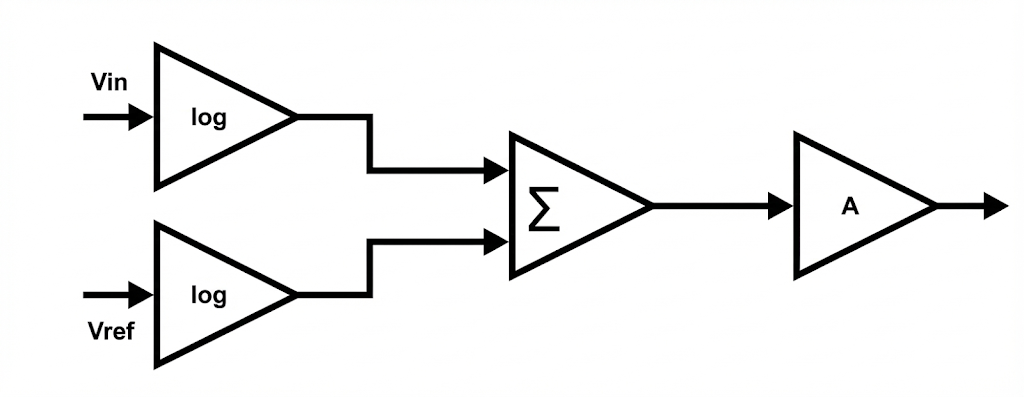
\includegraphics[width=0.5\linewidth]{Imagenes/1.17.png}
    \caption{}
    \label{fig:1.17}
\end{figure}
Esta última muestra que la tensión de cruce queda definida por la tensión de referencia y, además, si la ganancia del amplificador lineal ($A$) se hace dependiente de la temperatura de modo que compense el efecto de $V_t$, también se estabiliza la pendiente ($V_y$).

Intercambiando las posiciones de la resistencia y el transistor mostradas en la Fig.~1.15, se realiza la función inversa (exponencial) Fig.~1.18. En efecto, con los mismos argumentos utilizados en el amplificador logarítmico, se deduce para la tensión de salida la siguiente expresión:

\begin{equation}
    V_o = -I_C \cdot R_2 = -R_2 \cdot I_S \cdot e^{\frac{V_{in}}{V_t}} = V'_{ref} \cdot e^{\frac{V_{in}}{V_t}} \label{eq:1.21}
\end{equation}
\begin{figure}[H]
    \centering
    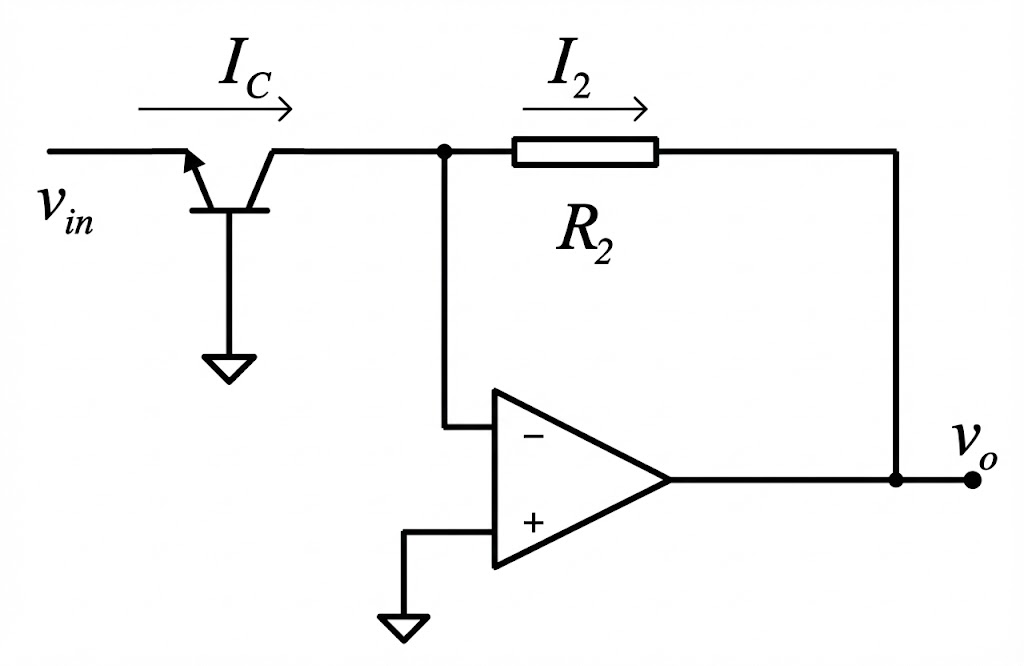
\includegraphics[width=0.5\linewidth]{Imagenes/1.18.png}
    \caption{}
    \label{fig:1.18}
\end{figure}
La relación exponencial de la tensión de salida respecto de la señal de entrada muestra la característica expansora de este amplificador, esto se aprecia mas claramente en una gráfica logarítmica donde la relación de transferencia vuelve a ser una línea recta de pendiente 0.433 $dec/Vt$..

\begin{equation}
\log(V_{0e}) = V_{ref} + \left(\frac{V'_{in}}{Vt}\right).\log(e) \tag{1.22}
\end{equation}

Si la señal de entrada de este amplificador ($V'_{in}$), es la de salida del logarítmico compensado dada en (1.20), ($V'_{in}= V_{0L}$), a partir de la anterior se deduce que la señal de salida ($V_{0e}$), recupera la de entrada ($V_{in}$), a menos de una constante. En efecto en el \underline{log} se verifica que:

\[
V_{0L} = -Vt.Ln\left(\frac{V_{in}}{V_{ref}}\right) \Rightarrow V_{in} = -R_{1}.I_{S}.e^{\left(\frac{V_{0L}}{Vt}\right)}
\]

Comparando la anterior con (1.21) se obtiene para $V'_{in} = V_{0L}$
Una fuente de tensión independiente real, puesta en el lazo, en serie con el generador controlado de salida del O.A., tiene un efecto nulo sobre la tensión de salida en condiciones de operación ideales.

La Figura \ref{fig:1.19}a, muestra un amplificador ideal, excitado por el generador $v_1$ con resistencia interna $r$ que está inserta en el lazo. Para demostrar lo afirmado se analizará en forma independiente el efecto sobre $v_o$ producido por la tensión ($v_1$) y el de $r$ sobre la impedancia vista desde la salida ($r_{of}$).

La \ref{fig:1.19}b muestra el circuito en lazo abierto para evaluar el primero a través de la GLC producida por $v_1$ utilizando la fórmula de Black y para calcular $r_{of}$ mediante la respectiva de Blackman.
\begin{equation}
V_{in} = \left(\frac{R_{1}}{R_{2}}\right).V_{0e} \tag{1.23}
\end{equation}
\subsubsection{Rectificador de precisión}
\begin{figure}[H]
    \centering
    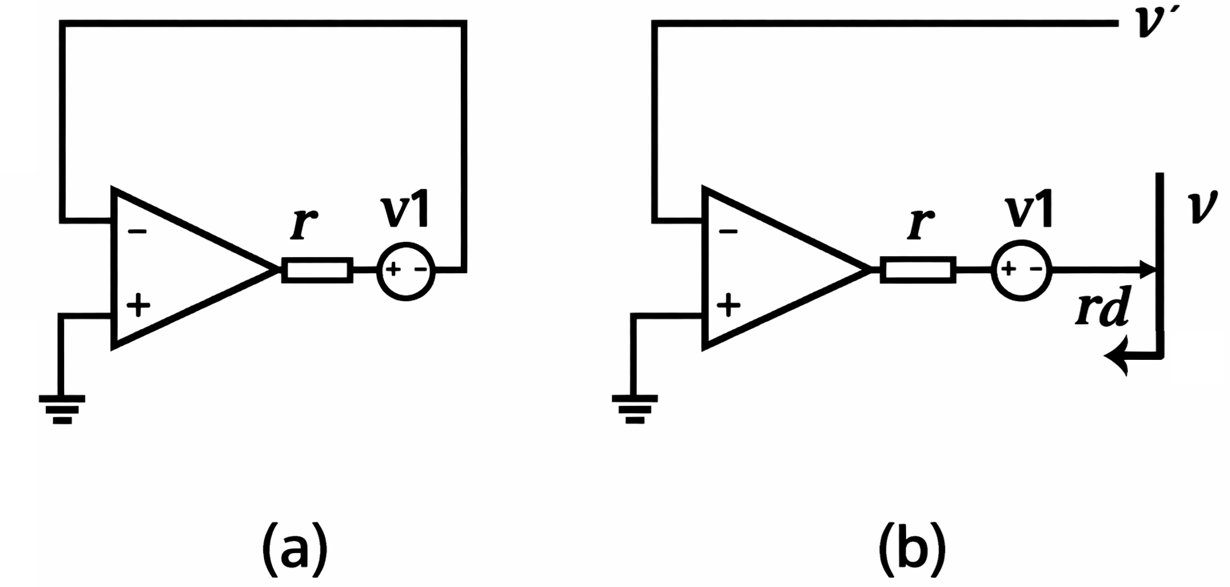
\includegraphics[width=0.5\linewidth]{Imagenes/1.19.png}
    \caption{Realimentacion del amplificador}
    \label{fig:1.19}
\end{figure}
Para el primer caso se deducen las siguientes relaciones para el cálculo de GLC.

\[
\left. G_{LA} \right|_{v=0} = \frac{v_0}{v_1} = -1 \quad \text{y} \quad \left. T \right|_{v_1=0} = \frac{v_0}{v} = -A_d
\]

Luego la ganancia de lazo cerrado es

\begin{equation}
\left. A_{vf} \right|_{A_d \to \infty} = \frac{v_o}{v_1} = \frac{G_{LA}}{(1 - T)} = \frac{-1}{1 + A_d} = 0 \tag{1.24}
\end{equation}

Para el cálculo de la impedancia se deben conocer la del sistema muerto ($r_o$) y las ganancias de lazo con la sección de interés en cortocircuito ($T_{cc}$) y en sección abierta ($T_{ca}$), con los generadores independientes pasivados.

De la figura \ref{fig:1.19}b se deduce además que la impedancia de sistema muerto ($v' = v_I = 0$) es igual a la resistencia interna del generador $v_1$.

\[
r_0 = r
\]

Es fácil ver que la ganancia de lazo, con la sección en cortocircuito es nula

En efecto si: $v_o = 0 \implies T_{cc} = \frac{v'}{v} = 0$
Para el primer caso se deducen las siguientes relaciones para el cálculo de GLC.

\[
\left. G_{LA} \right|_{v=0} = \frac{v_0}{v_1} = -1 \quad \text{y} \quad \left. T \right|_{v_1=0} = \frac{v_0}{v} = -A_d
\]

Luego la ganancia de lazo cerrado es

\begin{equation}
\left. A_{vf} \right|_{A_d \to \infty} = \frac{v_o}{v_1} = \frac{G_{LA}}{(1 - T)} = \frac{-1}{1 + A_d} = 0 \tag{1.24}
\end{equation}

Para el cálculo de la impedancia se deben conocer la del sistema muerto ($r_o$) y las ganancias de lazo con la sección de interés en cortocircuito ($T_{cc}$) y en sección abierta ($T_{ca}$), con los generadores independientes pasivados.

De la \ref{fig:1.19}b se deduce además que la impedancia de sistema muerto ($v' = v_I = 0$) es igual a la resistencia interna del generador $v_1$.

\[
r_0 = r
\]

Es fácil ver que la ganancia de lazo, con la sección en cortocircuito es nula

\[
\text{En efecto si: } v_o = 0 \implies T_{cc} = \frac{v'}{v} = 0
\]

En cambio con la sección en circuito abierto aquella resulta:

\[
T_{ca} = \frac{v'}{v} = -A_d
\]

Finalmente la impedancia en lazo cerrado es:

\begin{equation}
\left. r_{0f} \right|_{A_d \to \infty} = \frac{r_0}{1 - T_{ca}} = \frac{r_0}{1 + A_d} = 0 \tag{1.25}
\end{equation}

Las conclusiones anteriores permiten afirmar, que un diodo puesto en el lazo como indica la \ref{fig:1.20}a, tiene un comportamiento cuasi ideal, permitiendo en consecuencia rectificar con precisión señales del orden de las decenas de microvoltios.
\begin{figure}[H]
    \centering
    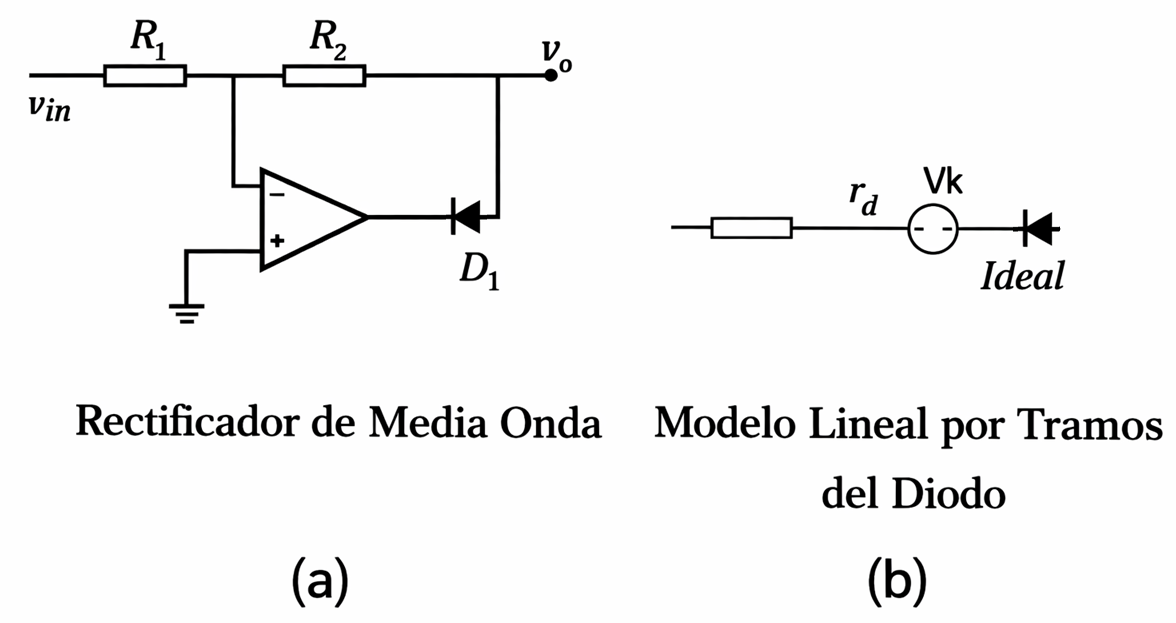
\includegraphics[width=0.5\linewidth]{Imagenes/1.20.png}
    \caption{Modelo lineal del rectificador}
    \label{fig:1.20}
\end{figure}
En efecto si el diodo real es reemplazado por el modelo lineal por tramos de \ref{fig:1.20}b y polarizando directamente el diodo ideal ($v_{in} > 0$), tanto la tensión de codo ($V_K$), como la resistencia dinámica ($r_d$) son reducidas por la ganancia de lazo, según (1.24) y (1.25), tal que en condiciones ideales son anuladas, resultando en consecuencia válido para el semiciclo positivo de la señal.

En cambio en el semiciclo negativo de esta última, el diodo queda polarizado inversamente abriendo el lazo de realimentación respectiva y la salida satura hacia la tensión de alimentación de la barra positiva.

Para evitar esto, se conecta un segundo diodo $D_2$ (\ref{fig:1.21}), que enclava la excursión a $-0.7V$ aproximadamente. Es obvio que invirtiendo la conexión de los diodos de \ref{fig:1.21}, el circuito rectificaría el semiciclo negativo de la señal de entrada.
\begin{figure}[H]
    \centering
    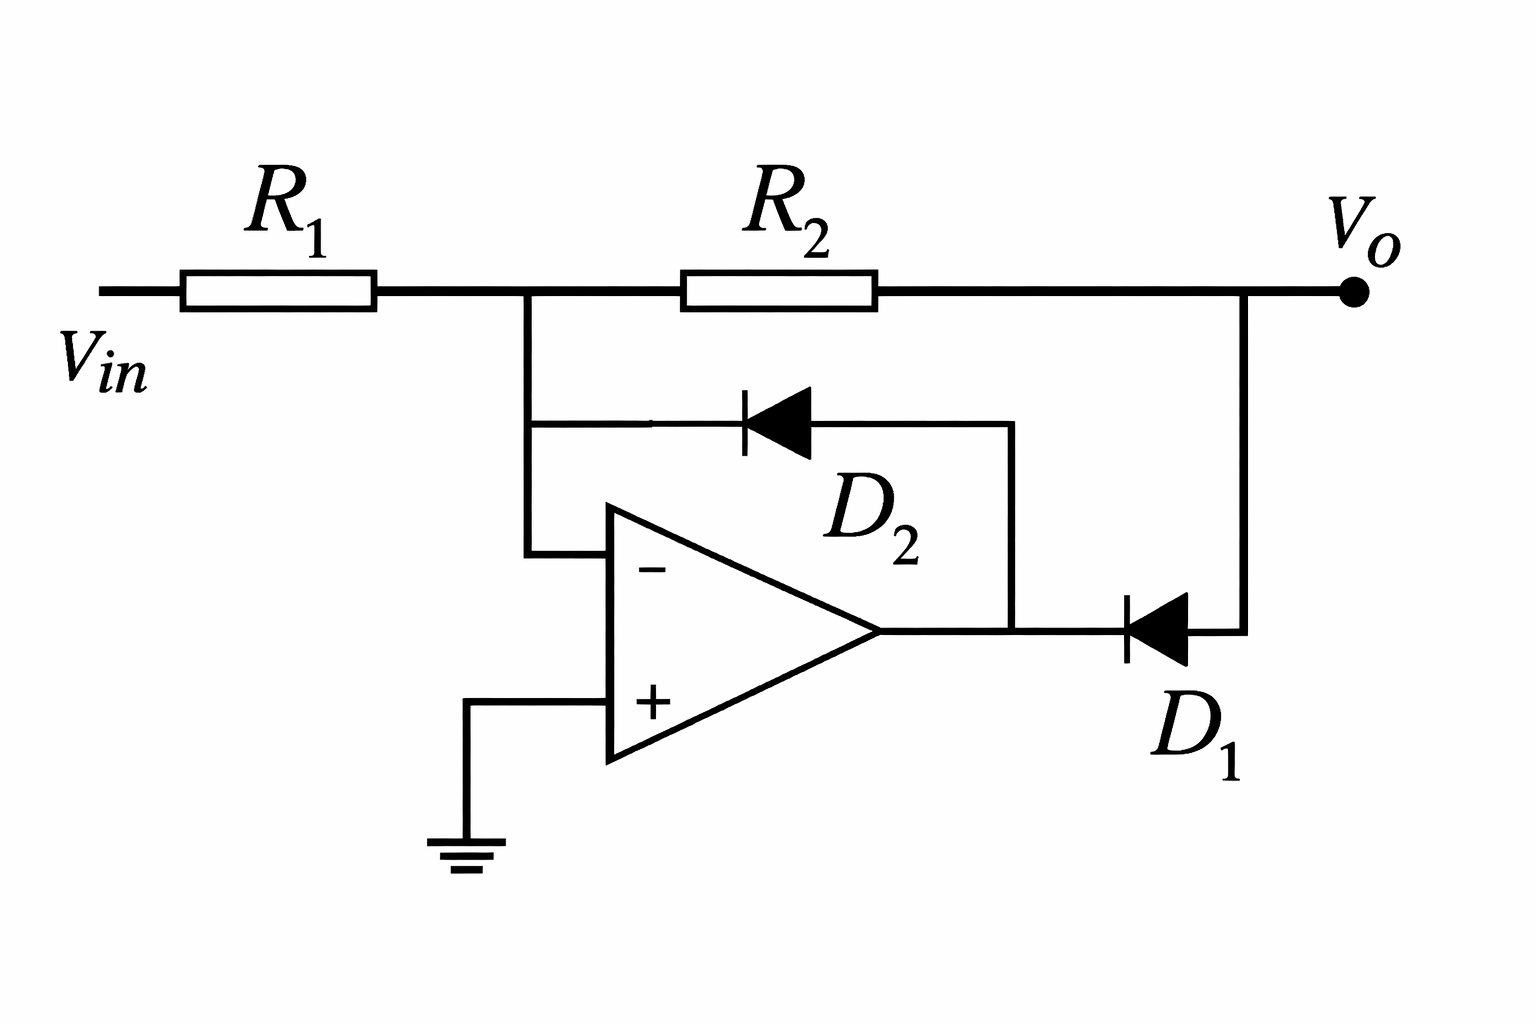
\includegraphics[width=0.5\linewidth]{Imagenes/1.21.png}
    \caption{ Circuito con Enclavamiento }
    \label{fig:1.21}
\end{figure}
No obstante el ejemplo que se analiza a continuación corresponde a una aplicación lineal es oportuno destacar que los conceptos anteriores son aplicables también al diodo base emisor del transistor $Q_n$ y $Q_p$ dentro del lazo de los circuitos de \ref{fig:1.22}.

En efecto, (a) configura una fuente de corriente unipolar controlada por tensión que alimenta la carga $R_L$. El conjunto opera como un amplificador separador (Buffer) con la disponibilidad de corriente de salida del A.O, multiplicada por la ganancia del transistor ($h_{FE}$).

En (b) la conexión configura un amplificador de simetría complementaria en el que debido al comportamiento ideal de las juntas, se elimina la distorsión de cruce, (Clase B ideal), e igual que el caso anterior se aumenta la capacidad de suministro de corriente del A.O a la carga, (Booster de Corriente).

Del esquema (a) se deduce el siguiente valor de la corriente en la carga.

\[
I_L = I_C = \frac{V_{in}}{R_L} \qquad \text{para } v_{in} > 0
\]

De igual manera en (b) para ambas polaridades de la señal de entrada.
\begin{figure}[H]
    \centering
    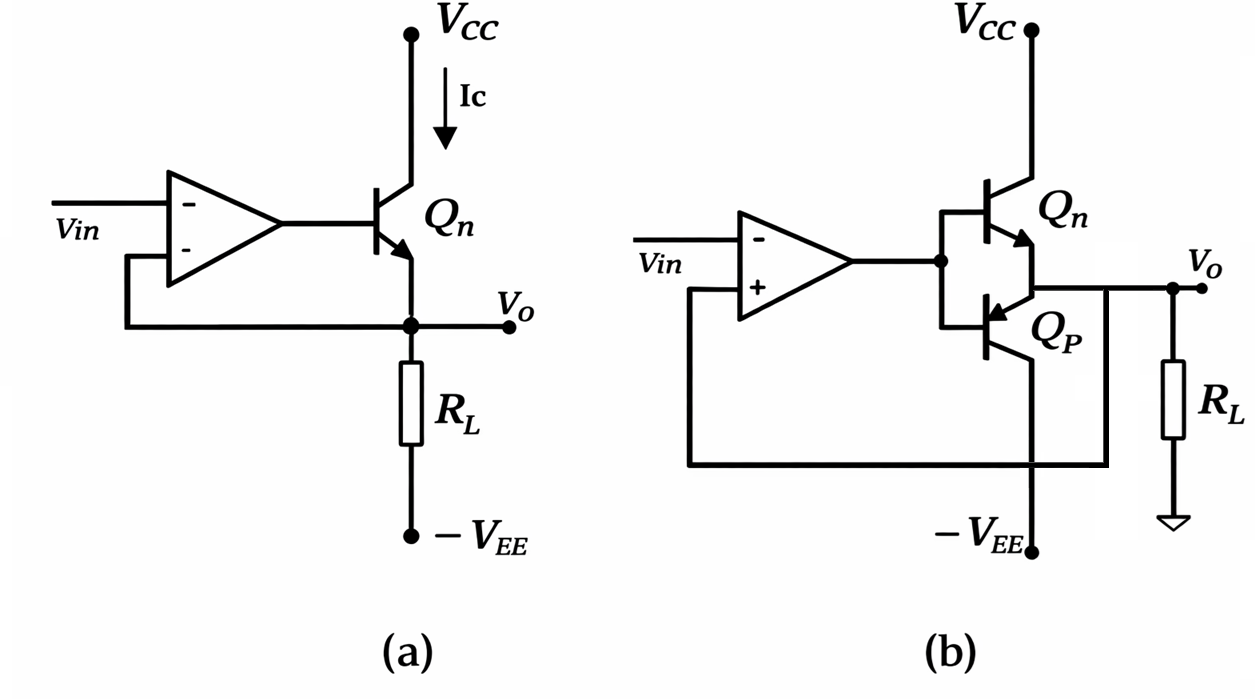
\includegraphics[width=0.5\linewidth]{Imagenes/1.22.png}
    \caption{}
    \label{fig:1.22}
\end{figure}
\subsection{Problemas unidad 1}
\textbf{P.1.1} Calcular las impedancias vistas por el generador de señal y la carga ($z_{in}$, $z_o$), en las configuraciones básicas de \ref{fig:1.5} y \ref{fig:1.6}

\textbf{P.1.2} En el esquema adjunto, el fotodiodo convenientemente iluminado se comporta como una fuente de corriente operando en cortocircuito. El amplificador convierte la corriente del fotodiodo en una tensión proporcional de salida. Deducir la relación de transferencia ideal ($v_o/I_f$) y la impedancia vista por el generador de señal. Considere $r_d = \infty$ y $c_d = 0$.
\begin{figure}[H]
    \centering
    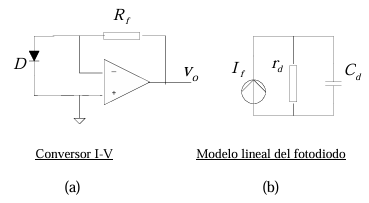
\includegraphics[width=0.5\linewidth]{Imagenes/1.23.png}
    \caption{}
    \label{fig:1.23}
\end{figure}
\textbf{P 1.3} El amplificador diferencial tiene extensa aplicación en acondicionadores de señales analógicas (Instrumentación). Los esquemas siguientes muestran algunas configuraciones típicas y en referencia a ellas desarrollar los siguientes ítems:

\textbf{Config. a)} Encontrar las siguientes relaciones:

\[
v_{o1} = f(v_1, v_2), \quad v_{o2} = f(v_1, v_2), \quad (v_{o2} - v_{o1}) = f(v_1, v_2), \quad \frac{v_{o2} + v_{o1}}{2} = f(v_1, v_2)
\]

\begin{figure}[H]
    \centering
    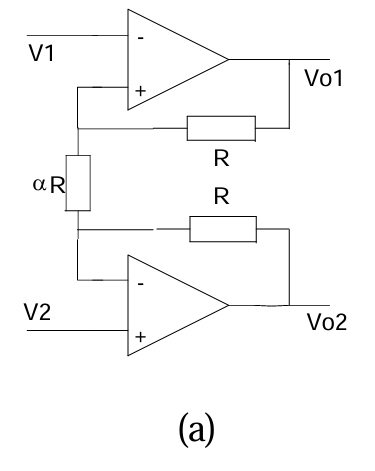
\includegraphics[width=0.5\linewidth]{Imagenes/1.24.png}
    \caption{}
    \label{fig:1.24}
\end{figure}
\textbf{Config. b y c .)} Deducir la ganancia de modo diferencial ($v_o / (v_2 - v_1)$).
\begin{figure}[H]
    \centering
    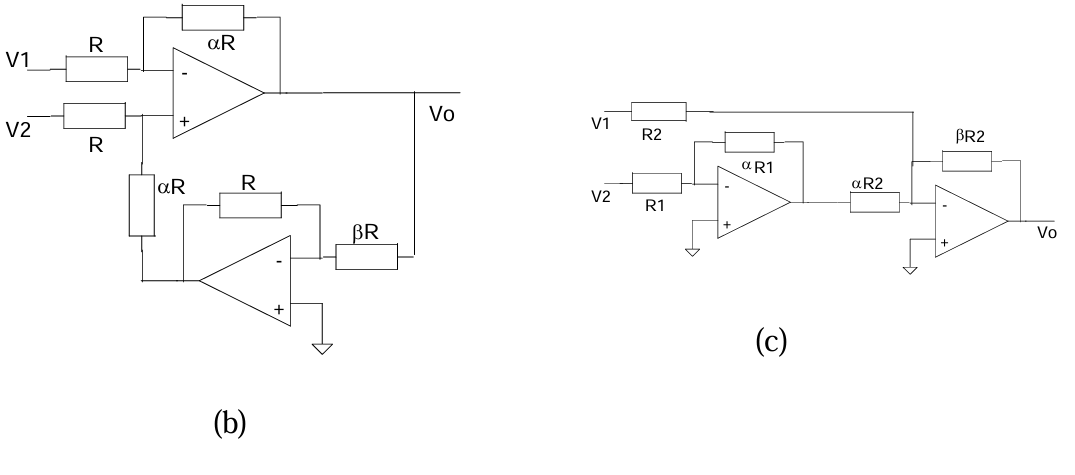
\includegraphics[width=0.85\linewidth]{Imagenes/1.25.png}
    \caption{}
    \label{fig:1.25}
\end{figure}
\textbf{P1.4} Calcular la ganancia de modo diferencial de la configuración resultante de conectar el amplificador de \ref{fig:P1.3}a como excitador del de \ref{fig:1.6}.

\textbf{P.1.5.} Diseñar un amplificador de corriente alterna (\ref{fig:1.7}), con las siguientes características: Ganancia en la banda de paso $(v_o /v_{in}) = -2$, frecuencia de corte en bajas frecuencias $f_L = 1\text{kHz}$.

\textbf{P.1.6.} Diseñar un conversor I-V (\ref{fig:P1.2}) cuyo fondo de escala debe ser de $10\text{V}$ cuando es excitado por un fotodiodo que opera en modo fotovoltaico ($V_d=0$) y debe convertir la corriente mínima de $30\text{pA}$ en $30\mu\text{V}$.

\textbf{P.1.7} Determinadas aplicaciones exigen valores de la resistencia de realimentación muy elevadas penalizando severamente su operación. El resultado del problema 1.6, es un ejemplo. Una solución frecuente y práctica es simular la alta impedancia de realimentación requerida, mediante un cuadripolo como el indicado en \ref{fig:P1.7}. Se pide:

\begin{enumerate}
    \item[a)] Deducir la relación de transferencia, $(V_o / I_f)$, del conversor con el reemplazo indicado en la figura respectiva.
    \item[b)] Calcular un juego de valores de las resistencias donde ninguna supere los $100\text{k}\Omega$, para simular el valor calculado en P1.6.
\end{enumerate}
\begin{figure}[H]
    \centering
    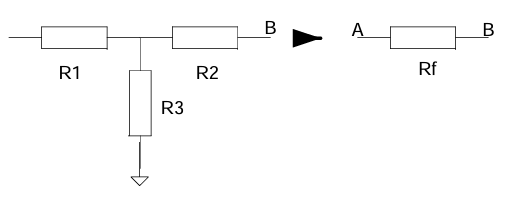
\includegraphics[width=0.5\linewidth]{Imagenes/1.26.png}
    \caption{}
    \label{fig:1.24}
\end{figure}
\textbf{P.1.8.} La fuente de corriente controlada por tensión de \ref{fig:1.11} utiliza el AO-LM324 alimentado por $\pm 10\text{V}$ con los siguientes valores de componentes: $R_1 = R_2 = 10\text{k}\Omega$, $R_3 = R_4 = 600\Omega$, $R_L = 10\text{k}\Omega$, $V_{in} = 25\text{mV}$.

Calcular la tensión en la carga ($R_L$), a la salida del amplificador ($V_o$) y las corrientes circulantes en todas las resistencias para los siguientes valores de la impedancia de carga: $R_L = 0\Omega$; $5\text{k}\Omega$ y $R_{Lmax}$.

Comente los resultados.

\textbf{P.1.9} Si en el problema anterior, el amplificador estuviere alimentado con tensión partida ($\pm 12\text{V}$). ¿Cuál sería el valor de resistencia de carga máxima admitida? Explique.

\textbf{P.1.10} El circuito involucrado en P.1.9 puede funcionar como Óhmetro. Explique.

\textbf{P.1.11} El circuito de la figura es un rectificador de media onda de precisión. Graficar la función de transferencia $V_{out}=f(V_{in})$. En base a lo demostrado en la sección 1.3, considere ideales los diodos.

Sugerencia: analizar separadamente para $V_{in} > 0$ y $V_{in} < 0$.
\begin{figure}[H]
    \centering
    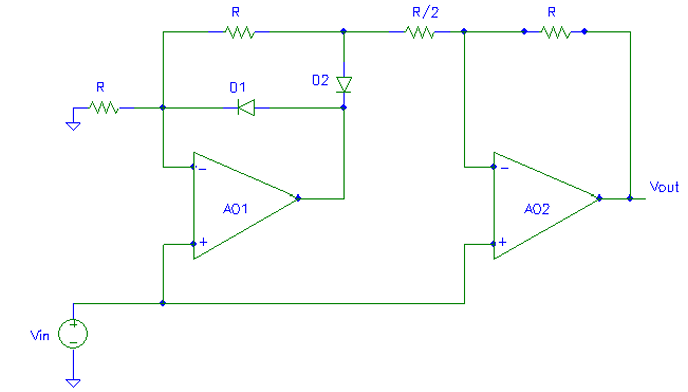
\includegraphics[width=0.5\linewidth]{Imagenes/1.27.png}
    \caption{}
    \label{fig:1.27}
\end{figure}
\textbf{P1.12} Repita el análisis de P1.11, excitando el nodo inversor de $AO_1$, a través de la resistencia $R$.

\textbf{P 1.13} Repita el análisis de P1.12, con el agregado de una resistencia de valor $R$ conectada entre el terminal positivo del generador de señal y la entrada inversora de $AO_2$.

\textbf{P1.14.} El circuito de la figura, opera con ganancia variable por tramos. $AO_1$ es un amplificador operacional ideal. $Z_1$ y $Z_2$ son diodos Zener de $5\text{V}$, $Z_3$ y $Z_4$ de $8\text{V}$. Graficar $V_{out}$ vs $V_{in}$, cuando esta última varía entre $V_{SS}$ y $V_{CC}$. Indicar en el diagrama las coordenadas de los puntos singulares.
\begin{figure}[H]
    \centering
    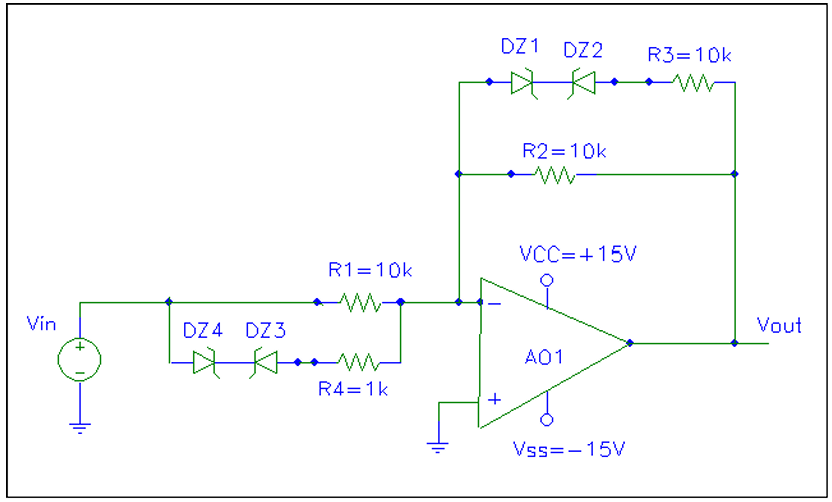
\includegraphics[width=0.5\linewidth]{Imagenes/1.28.png}
    \caption{Enter Caption}
    \label{fig:1.28}
\end{figure}